\chapter{面向微博的反讽识别}
\label{cha:exp_irony_det}

\section{本章引论}

社交媒体的发展对我们的语言体系带来了很大的影响,网络上出现了很多新颖的用词和句式,语言的表达方式越来越丰富,也越来越复杂。而反讽是在网络上常见的语言修饰手法之一, 这为反讽相关的研究带来了充足的数据基础。Henry Watson Fowler在《The King's English》一书中指出反讽的使用使得“表面意思和实际意思不同”。譬如一个人说“你这想法真有创意”,在字面意思上是对另一个人的赞同,但在特定背景下,如后接一句“你真相信这能实现吗”,那么发言者实际上可能暗示这个想法无法落地,表面上称赞为“有创意”,其实是指责这种想法不切实际。这在意图识别当中尤其重要,忽略反讽的使用会导致对内容的错误理解,而且这种理解是和真实意思截然相反的,因此识别出反讽的使用或许对相关的场景如情感识别、人机交互能起着正面的作用。

根据Joshi等人\cite{joshi2017automatic}对近年相关研究的总结,反讽识别可以大致分成基于规则的方法和基于机器学习的方法。基于规则的方法透过人工找出反讽中的语言规律,设计出对应的模式,然后在新样本中尝试识别出相应的模式出现。和机器学习方法对比,基于规则的方法优点在于无需模型训练,但要求研究员对反讽有充分的语言理解,设计的模式对样本的复盖程度决定了算法的识别能力。而随着近年深度学习快速发展,一些研究更专注于对词嵌入向量的使用以及人工神经网络的设计和选择。

国际比赛SemEval-2018的任务三\cite{van2018semeval}旨在促进英语微博中的反讽识别研究,其中包含了两个子任务。子任务一是二分类的反讽识别,需要识别微博是否有使用反讽。子任务二是四分类的反讽识别,是子任务一的拓展,除了判断微博是否包含反讽,反讽再细分成三个类别:基于相反语义的反讽 
、情景反讽、其他反讽。本章节中我们将基于SemEval-2018的任务三进行实验,采用比赛组织者提供的训练数据和测试数据,并透过和其他参赛系统进行比较来评估我们提出的框架的性能。

本章的内容安排如下。在章节\ref{sec:exp_irony_det_format}中,我们会基于章节\ref{sec:global_problem_analysis}首先给出当前问题的形式化表示。在章节\ref{sec:exp_irony_det_data}中我们再对具体实验数据进行观察,分析微博文本的特性以及各个反讽类别之间的不同。在章节\ref{sec:exp_irony_det_framework}中,我们会基于章节\ref{sec:global_framework}的框架给出我们对当前问题的系统框架。最后在章节\ref{sec:exp_irony_det_exp}给出实验的细节,以及对实验结果进行分析。

\section{形式化表示}
\label{sec:exp_irony_det_format}

在本章中,我们要研究单条微博的反讽类型识别。给定一个反讽类别集合$C$,对于一个微博集合$T$,对任意一条微博$t \in T$,它属于唯一一种情感类别$c \in C$。又给定一个词集合$W$,微博$t$经过文本预处理后可以表示为一个长度为$L$的词序列 $w = <w_1, w_2, ..., w_L>, w_i \in W, i \in [1, L]$。因为没有引入上下文信息,所以背景$B$在模型中忽略。那么我们的目标是找出一个映射关系$F_C$,使得$c=F_C(w)$。

\section{数据观察}
\label{sec:exp_irony_det_data}

我们的实验完全采用SemEval-2018的任务三比赛组织者提供的数据集,其中的语料收集自微博平台Twitter上发布于2014年至2015年之间的微博,再由人工标注得出每条微博的反讽类型。该比赛的两个子任务均采用了相同的语料但标注稍有不同。子任务一是二分类的反讽识别,需要识别微博是否有使用反讽,各类别的数据分布如表\ref{tab:semeval_2018_task3_A_data}所示,表\ref{tab:semeval_2018_task3_A_sample}为语料中两个类别的例子。可以看出没有反讽和带有反讽两个类别的样本在训练集上大致比例为1:1,在测试集上两个类别的分布大致为3:2。

\begin{table}[htb]
  \centering
  \begin{minipage}[t]{0.7\linewidth} % 如果想在表格中使用脚注,minipage是个不错的办法
  \caption{反讽识别子任务一各类别样本数量分布}
  \label{tab:semeval_2018_task3_A_data}
    \begin{tabularx}{\linewidth}{X|XX}
    \toprule[1.5pt]
    数据集 & 没有反讽 & 带有反讽 \\  
    \hline
    训练集 & 1923 & 1911 \\
    测试集 & 473  & 311 \\
    \bottomrule[1.5pt]
    \end{tabularx}
  \end{minipage}
\end{table}

\begin{table}[htb]
  \centering
  \begin{minipage}[t]{0.8\linewidth} % 如果想在表格中使用脚注,minipage是个不错的办法
  \caption{反讽识别子任务一样例}
  \label{tab:semeval_2018_task3_A_sample}
  \begin{tabularx}{\linewidth}{l|X}
    \toprule[1.5pt]
    反讽类别 & 例子 \\
    \hline
    没有反讽 & Had no sleep and have got school now \#not happy \\
    带有反讽 & I just love when you test my patience!! \#not \\
    \bottomrule[1.5pt]
  \end{tabularx}
  \end{minipage}
\end{table}

子任务二是四分类的反讽识别,是子任务一的拓展,除了判断微博是否包含反讽,反讽再细分成三个类别:基于相反语义的反讽(在部分图表中将简称为“反义反讽”)、情景反讽、其他反讽。各类别的数据分布如表\ref{tab:semeval_2018_task3_B_data}所示,表\ref{tab:semeval_2018_task3_B_sample}为语料中各反讽类别的例子。可以看出带有反讽一类细分成三个子反讽类别后各个类别的分别变得明显的不均匀,三个子反讽类别中的样本数据量差异也较大,基于相反语义的言语反讽占了其中一半以上,在模型训练过程应有对应策略处理。

\begin{table}[htb]
  \centering
  \begin{minipage}[t]{\linewidth} % 如果想在表格中使用脚注,minipage是个不错的办法
  \caption{反讽识别子任务二各类别样本数量分布}
  \label{tab:semeval_2018_task3_B_data}
    \begin{tabularx}{\linewidth}{X|XXXX}
    \toprule[1.5pt]
    数据集 & 没有反讽 & 基于相反语义的反讽 & 情景反讽 & 其他反讽\\  
    \hline
    训练集 & 1923 & 1390 & 316  & 205 \\
    测试集 & 473  & 164  & 85  & 62 \\
    \bottomrule[1.5pt]
    \end{tabularx}
  \end{minipage}
\end{table}

\begin{table}[htb]
  \centering
  \begin{minipage}[t]{\linewidth} % 如果想在表格中使用脚注,minipage是个不错的办法
  \caption{反讽识别子任务二样例}
  \label{tab:semeval_2018_task3_B_sample}
  \begin{tabularx}{\linewidth}{l|X}
    \toprule[1.5pt]
    \small 反讽类别 & 例子 \\
    \hline
    \small 没有反讽 & Had no sleep and have got school now \#not happy \\
    \small 基于相反语义的反讽 & \small I really love this year’s summer; weeks and weeks of awful weather \\
    \small 情景反讽 & Most of us didn’t focus in the \#ADHD lecture. \#irony \\
    \small 其他反讽 & @someuser Yeah keeping cricket clean, that's what he wants \#Sarcasm \\
    \bottomrule[1.5pt]
  \end{tabularx}
  \end{minipage}
\end{table}

比赛组织者对四种反讽类别给出了对应的说明。对基于相反语义的反讽一类,文本中存在某部分内容表达了可评估的情感极性,但整条微博实际上表达了相反的情感极性。如表\ref{tab:semeval_2018_task3_B_sample}中的例子,“love”在字面意思上表达了正面的情感,但微博后半中“awful weather”提示实际情况引起了发言者的不适,发言者其实在表达对这个夏天坏天气的不满,这和“love”的正面情感恰恰相反。对于情景反讽一类,文本正描述某个场景,其中发生的事情和某种预期不符。如表\ref{tab:semeval_2018_task3_B_sample}中的例子,描述了一个参与讲座的场景,但“我们(us)”并没有专注于这场讲座,和“参与者应该专注于讲座内容”的预期相反。对于其他反讽一类,文本表达了讽刺的意思,但文本的字面意思和发言者表达的意思之间并不存在情感极性的反差。如表\ref{tab:semeval_2018_task3_B_sample}中的例子,发言者表示某人想要保持蟋蟀干净,字面上并不存在情感极性,但在句子后的井号标签提示了发言者表达了讽刺,认为“保持蟋蟀干净”是一样莫名奇妙的事情。最后是没有反讽一类,对于明显不可能包含反讽的文本,或者在背景信息不足的情况下不能确认其包含反讽的文本均属于这一类。

\subsection{文本长度}

我们首先对数据集的文本经过简单分词后统计各个类别的样本中词数量的分布,以下简称为文本长度。表\ref{fig:semeval2018_task3_train_class_len}和表\ref{fig:semeval2018_task3_test_class_len}分别显示了训练集和测试集上各类别样本的文本长度。综合先见样本的文本长度不超过了50,样本的平均文本长度约为20个词。根据表\ref{fig:semeval2018_task3_train_class_len}我们可以看出“情景反讽”的样本整体的文本长度较其他类别的长,“没有反讽”和“基于相反语义的反讽”在文本长度分布上没有明显区别,“其他反讽”整体的文本长度则略高于前两者。再观察表\ref{fig:semeval2018_task3_test_class_len},同样地“没有反讽”和“基于相反语义的反讽”在文本长度分布上没有明显区别,“情景反讽”的文本长度略高于前两者,但不如训练集上明显。

\begin{figure}[H]
  \centering
  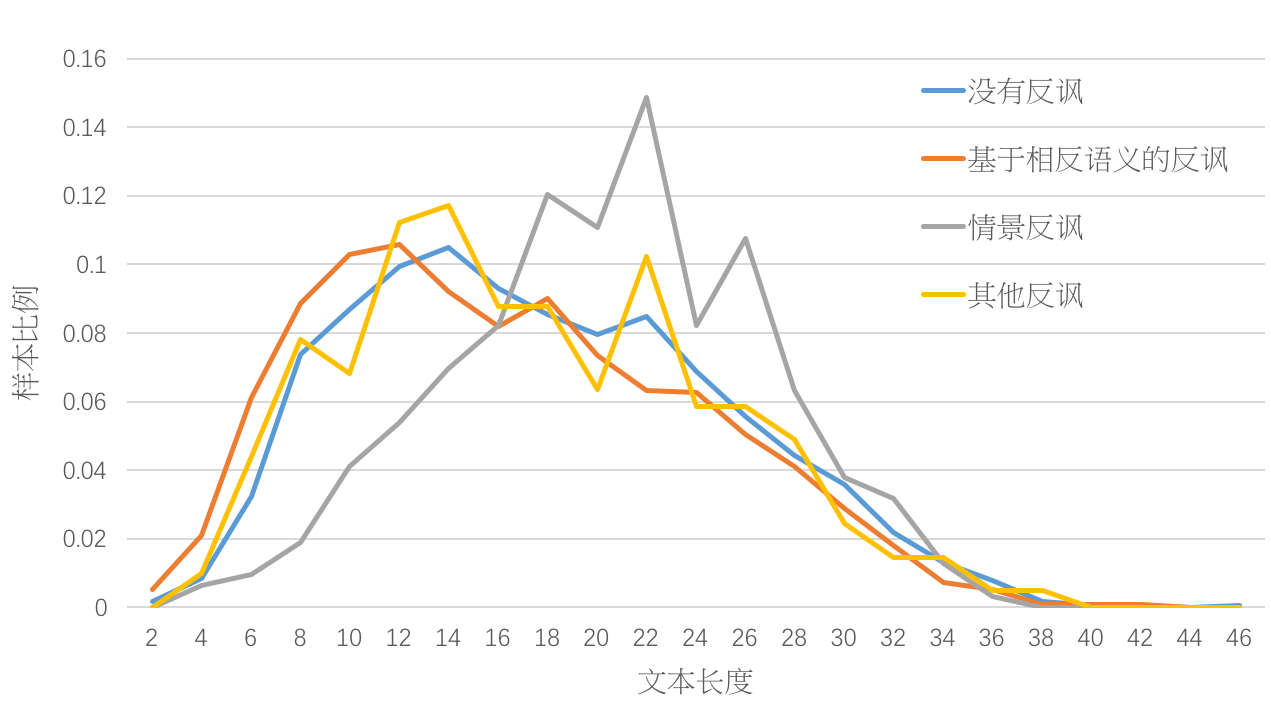
\includegraphics[width=\textwidth]{img/semeval2018_task3_train_class_len.png}
  \caption{反讽识别训练集上各类别文本长度分布}
  \label{fig:semeval2018_task3_train_class_len}
\end{figure}

\begin{figure}[H]
  \centering
  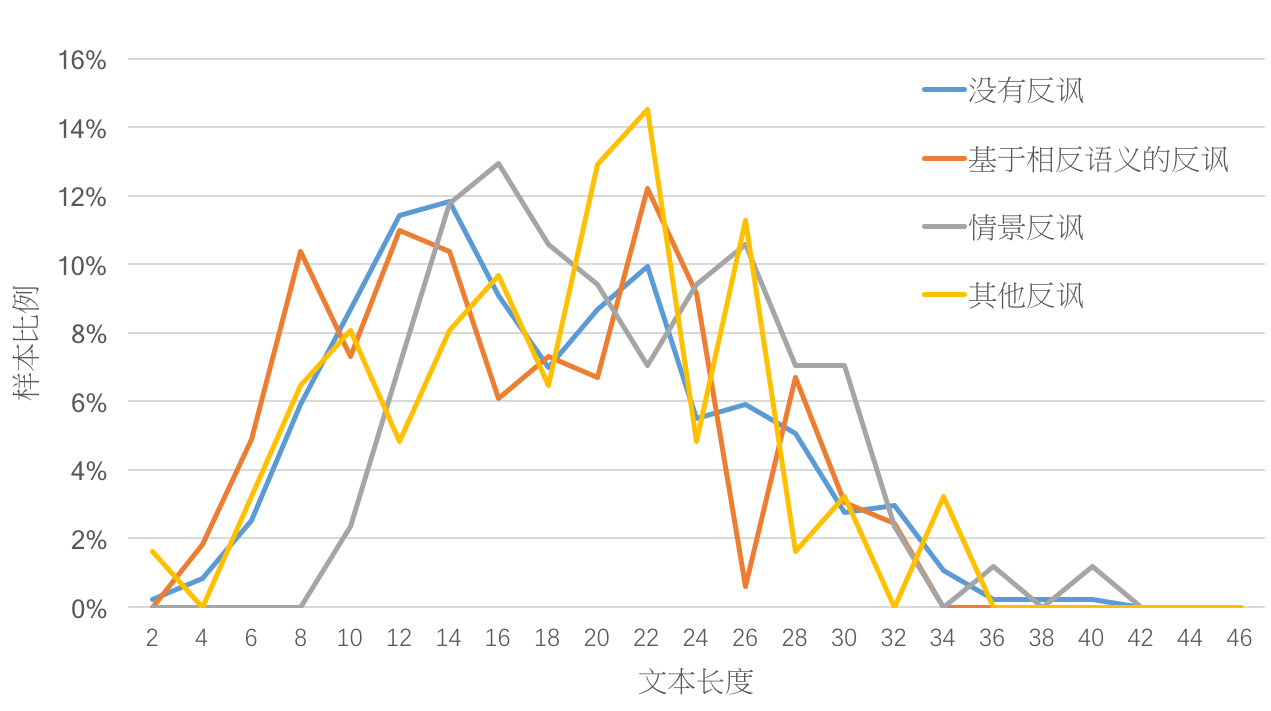
\includegraphics[width=\textwidth]{img/semeval2018_task3_test_class_len.png}
  \caption{反讽识别测试集上各类别文本长度分布}
  \label{fig:semeval2018_task3_test_class_len}
\end{figure}

\subsection{文本特征}
\label{ssec:exp_irony_det_data_text}

另外我们注意到语料中存在微博平台Twitter上特有的文本特征,出现频率较高的模式如下:

\begin{itemize}

\item 用户标签“@someuser”,对应微博上的一个用户,使用场景包括以下两种。一是作为句子中的名词使用,二是添加在句前或句末用于提示该用户的参与,不具有句法作用。

\item 井号标签“\#something”,使用场景大致分为以下两种。一是作为句子中的一部分,如“I \#do \#like \#it”,去除井号后满足正规的英语用法,此处以井号标签代替是对内容的强调。另一种是出现在句末,用于提示微博内容与标签对应内容相关,如句末出现“\#sarcasmtweet”明显表示讽刺。

\item 网站链接,在微博平台上支持附加一个网站链接以便,其中平台对链接进行了统一处理,在语料库中网站链接均形如“http://t.co/***”或“https://t.co/***”。

\item 转发标记“RT”(retweet),当用户转发某条微博并添加个人评论时,平台会自动在个人评论后附加转发的微博原文并以“RT”隔开。

\item 一些在社交媒体平台上常见的、有别于正规英语的用法,如拼写错误、缩略词、全大写字母的单词、表情符等,可以参考章节\ref{sec:text_preprocess}描述的例子。

\end{itemize}


\section{框架设计}
\label{sec:exp_irony_det_framework}

对于任务一,由于是二分类问题,我们的系统只包含一组二分类器,透过一次投票得出最终的预测结果,判断微博文本是否采用了反讽修辞。

对于任务二,我们提出的识别系统包含了四组分类器,分别面向不同的子分类问题,并依次经过四次投票结合各组分类器的预测结果来得出最终的预测结果。第一组分类器由$N_1$个四类分类器组成,对应原问题的四个类别。第二组分类器由$N_2$个二类分类器组成,用于区分“没有反讽”和“基于相反语义的反讽”两类。第三组分类器由$N_3$个二类分类器组成,用于区分“没有反讽”和“情景反讽”两类。第四组分类器由$N_4$个二类分类器组成,用于区分“没有反讽”和“其他反讽”两类。

对于一条待识别的微博,决策过程如下:

\begin{itemize}

\item 首先由第一组分类器内部进行多数投票得出$Label^{1}_{MV}$作为第一轮预测结果$Label_{I}$ 。为方便阅读,以下将对一组样本的第一轮预测结果称为中间结果一。

\item 第二步,由第二组分类器投票进行多数投票得出预测结果$Label^{2}_{MV}$,若超过$thr_{2}$分类器投票投给$Label^{2}_{MV}$且第一轮的预测结果$Label_{I}$为“没有反讽”或“基于相反语义的反讽”,则把预测结果修改为$Label^{2}_{MV}$,否则保持不变,以此得出第二轮的预测结果$Label_{II}$。为方便阅读,以下将对一组样本的第二轮预测结果称为中间结果二。

\item 第三步,由第三组分类器投票进行多数投票得出预测结果$Label^{3}_{MV}$,若超过$thr_{3}$分类器投票投给$Label^{3}_{MV}$且第二轮的预测结果$Label_{II}$为“没有反讽”或“情景反讽”,则把预测结果修改为$Label^{3}_{MV}$,否则保持不变,以此得出第三轮的预测结果$Label_{III}$。为方便阅读,以下将对一组样本的第三轮预测结果称为中间结果III。

\item 最后一步,由第四组分类器投票进行多数投票得出预测结果$Label^{4}_{MV}$,若超过$thr_{4}$分类器投票投给$Label^{4}_{MV}$且第三轮的预测结果$Label_{III}$为“没有反讽”或“其他反讽”,则把预测结果修改为$Label^{4}_{MV}$,否则保持不变,以此得出第四轮的预测结果$Label_{IV}$,同时作为整个系统对该微博的最终反讽识别结果。

\end{itemize}

整个决策过程可以分成两大部分。第一部分是初步完成对微博的四分类反讽识别,作为后续决策的基础,对应上述四步决策中的第一步。第二部分是基于第一部分的初步识别结果进行修正,对应上述四步决策中的后三步,每一步只关注被识别的两个类别的样本,由一组专门的子分类器重新给出识别结果,当新的结果充分可信则修改前一步得到的预测结果。在这里决策的可信度由投票数决定,当多数票由超过$thr$个分类器给出则认为充分可信。

\begin{figure}[H]
  \centering
  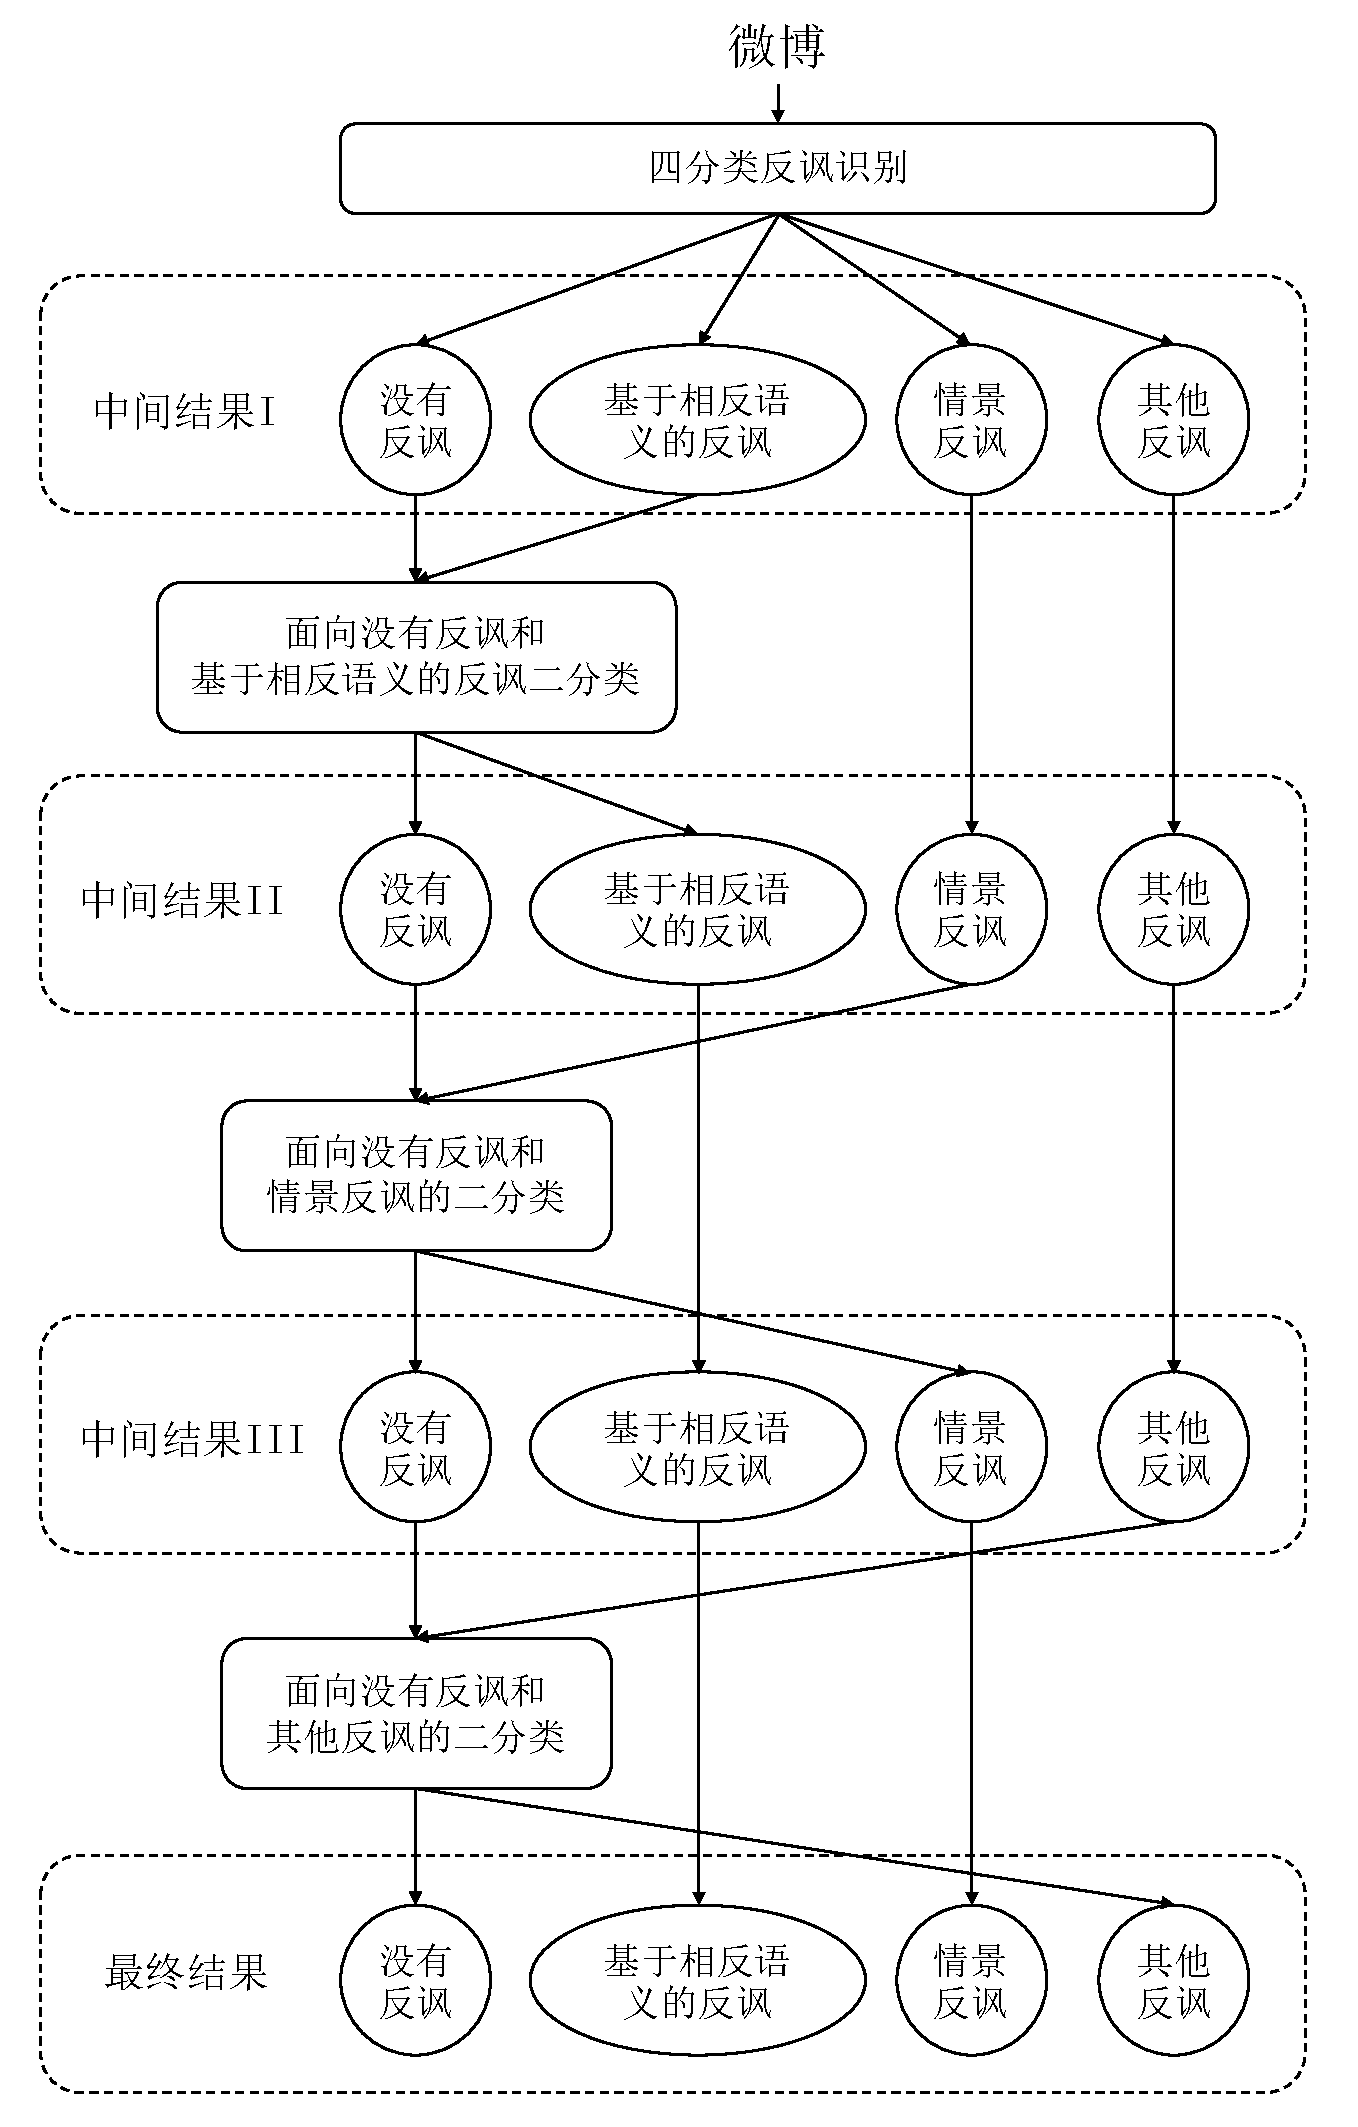
\includegraphics[width=0.9\textwidth]{img/irony_det_system.pdf}
  \caption{面向四分类反讽识别的系统框架}
  \label{fig:irony_det_system}
\end{figure}

其中对于每个子分类问题,我们都采用了相同的模型框架,如图\ref{fig:irony_det_cls_framework}所示,每个子分类器的输入都是微博文本经过预处理后得到的词序列$\{w_i\}$,然后每个词替换成对应的词嵌入向量,作为特征编码器的输入。特征编码器的目的是把微博文本对应的词向量序列转换成固定长度的特征向量,作为其反讽属性相关的表示向量,首先由一层或多层卷积神经网络或迭归神经网络组成,由于一维神经网络和迭归神经网络的输出均为和输入序列等同长度的向量序列,故最后需要再经过一层处理,对于迭归神经网络一般研究会取序列的最后一个向量,在理论上它结合了整段内容的信息,而对于迭归神经网络一般会采到最大池化层,分别取各特征位上的最大值,最后一种是采用注意力机制,对两类神经网络的序列输出均可结合成定长的表示向量。得到的表示向量作为后面概率预测器的输入,概率预测器的目的是基于微博定长的表示向量得出该微博属于各个反讽类别的概率分布,此处统一采用单层的全联接层和$Softmax$作为激活函数。最后取概率最高者作为分类器对该条微博预测的反讽类别。

考虑到对于不同反讽类型,其文本特征的提取方式可能有所不同,不同模型在各个子分类问题上的建模能力和识别性能也因此不同,所以对于每个子分类问题,我们会分别比较各组模型和参数的性能,以求在子分类问题上达到尽可能好的效果。

\begin{figure}[H]
  \centering
  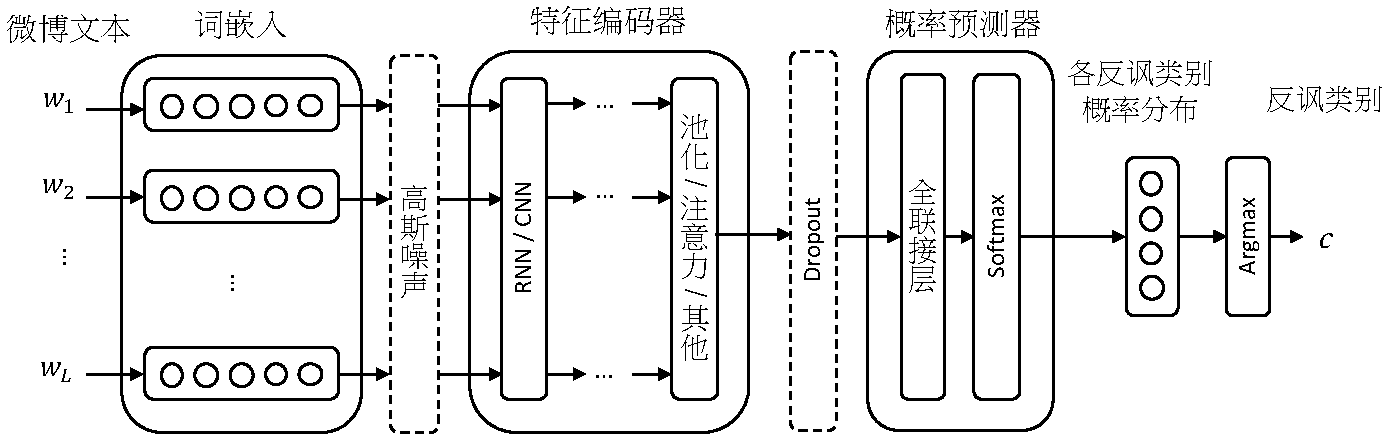
\includegraphics[width=\textwidth]{img/irony_det_cls_framework.pdf}
  \caption{反讽识别子分类器模型框架}
  \label{fig:irony_det_cls_framework}
\end{figure}

\section{实验与分析}
\label{sec:exp_irony_det_exp}

\subsection{数据预处理}

基于我们在章节\ref{ssec:exp_irony_det_data_text}中对样本文本的观察,我们依次采取了以下数据预处理手法

\begin{itemize}

\item 对于不用的用户标签“@someuser”,我们假设具体的用户名不影响微博内容的反讽类型,故统一替换成“<user>”。

\item 对于井号标签“\#something”,我们将他替换成一个字符串序列“<hashtag>”,“something”,“</hashtag>”,此处“<hashtag>”表示井号标签的开始,“</hashtag>”表示井号标签的结束,原因在于在Twitter平台上,井号标签可能由多个单词组成,如语料中出现的井号标签"\#SoCute",其内容应
砌解成“so”、“cute”两个单词,而语料中多单词组成的井号标签普遍以单词首字母大写示意,故可以简单完成分词,同时在前后添加“<hashtag>”和“</hashtag>”示意中间的内容属于同一个井号标签。

\item 全字母大写的内容在前后添加“<allcap>”和“</allcap>”,示意这一段文本可能是用户故意表示强调的内容。

\item 重复大于等次三次的标点符号以“<repeated>”示意,如“!!!”替换成序列“!”和“<repeated>”,表示“!”被多次重复以表达语气加强,同时假设重复次数不影响反讽的类型。

\item 将字母被故意重复的单词以“<elongated>”示意,如“Noooooooo”替换成序列“No”和“<elongated>”,表示“No”中某一个或多个字母被多次重复,但假设被重复的字符和重复的次数与反讽类型无关。

\item 将数字串替换成“<num>”,将电话号码替换成“<phone>”,将日期和时间分别替换成“<date>”和“<time>”,将数字百分比替换成“<percentage>”,超链接替换成“<url>”

\item 将由多个标点符号组成的表情符替换成对应的情感标签,如将“:)”替换成“<happy>”,将“:((”替换成“<sad>”。

\item 在完成以上处理后,对英文的大小写统一转换成小写。

\end{itemize}

以上功能我们利用了第三方的英语微博文本处理工具\textit{ekphrasis}\footnote{https://github.com/cbaziotis/ekphrasis}完成,对于其中如何分词、如何识别电话号码和日期、以及颜文字到情感标签的详细映射关系列表,读者可以直接参考其代码实现和配置文件。

\subsection{实验设置}

以下实验主要分成两大部分。第一部分是分析不同模型在不同子分类问题下的性能,根据章节\ref{sec:exp_irony_det_framework},我们最终的反讽识别框架涉及以下多个子分类问题:区分四个反讽类别的四分类问题、区分“没有反讽”和“基于相反语义的反讽”的二分类问题、区分“没有反讽”和“情景反讽”的二分类问题、区分“没有反讽”和“其他反讽”的二分类问题。对于各个子分类问题,我们基于章节~\ref{sec:exp_irony_det_framework}中的子分类模型框架进行实验,透过采用不同配置了解不同模型文本反讽识别的拟合能力。

第二部分是分析我们设计的识别系统的性能。我们会观察每一轮决策的调整如何改变局部的预测结果,而这些局部变化如何影响系统的整体性能。

%另外我们也会透过对设计的系统框架进行修改和比较,分析设计的合理性,以及当尝试将这种识别系统设计方式应用到其他场景时有哪些细节值得注意。

\subsection{评价指标}

按照国际比赛SemEval-2018任务三的设置,各个任务均以F1值作为识别系统性能的主要评价指标。对于其中一个类别$c$的F1值,其定义如下:

\begin{align}
  F_c = \frac{2 \times P_c \times R_c}{P_c + R_c} 
\end{align}

其中 $P_c$ 为类别$c$的正确率,$R_c$ 为类别$c$的召回率,其定义如下:

\begin{align}
  P_c &= \frac{TP_c}{TP_c + FP_c} \\
  R_c &= \frac{TP_c}{TP_c + FN_c}
\end{align} 

其中$TP_c$表示被系统预测为类别$c$,且真实标签为类别$c$的样本数量;$FP_c$表示被系统预测为类别$c$,但真实标签不是类别$c$的样本数量;$FN_c$被系统预测为不是类别$c$,但真实标签为类别$c$的样本数量。对于子任务一,系统性能以“带有反讽”一类样本的F1值为主要评估指标。对于子任务二,系统性能以各个类别的F1值的宏平均作为主要评价指标,即:

\begin{align}
  F1-macro = \sum\limits_{c \in C}F_c
\end{align}

此处$C$对应子任务二中四个类别组成的集合,即\{没有反讽,基于相反语义的反讽,情景反讽,其他反讽\}。在以下实验中,我们除了观察F1值、正确率和召回率,我们还会给出模型的准确率,其定义如下:

\begin{align}
  Acc &= \frac{\sum\limits_{c \in C} TP_c}{\sum\limits_{c \in C}(TP_c + FP_c)}
\end{align}

其中$TP_c$和$FP_c$如前述的定义,而$C$在子任务一中对应两个类别组成的集合,即\{没有反讽,带有反讽\}。

\subsection{模型训练}
\label{ssec:exp_irony_det_model_training}

对于不同的模型,我们都采用了以下策略来进行训练:

\begin{itemize}

\item 对于每个子分类器,在训练开始前我们先从每一类的训练样本中随机选出10\%的样本作为验证集,以此保留各个类的样本量分布。在每一轮模型训练中,学习算法基于另外90\%的训练样本对网络参数进行调整,然后计算模型在验证集上的F1值,经过有限轮迭代后,取在验证集上达到最优F1值的网络参数作为该子分类器最终的参数,以此缓解在训练数据上过拟合的问题。另外由于最终预测结合由多个子分类器投票联合得出,为了充分运用训练数据,每个分类器的验证集为独立随机筛选得出,一方面保证每个训练样本都有概率被用于某个分类器的参数调整,另一方面使得各个分类器的训练数据不同,因此对文本特征的建模也会有所不同,理论上对过拟合同样有缓解的作用,更有利于最后的投票。

\item 对于词嵌入层,我们利用了章节\ref{ssec:embedding}中提到的Baziotis等人\cite{baziotis2018ntua}提供的词嵌入模型,直接用于初始化词嵌入层的参数。在训练过程中,我们不对词嵌入层的参数进行调整。考虑到若允许词嵌入层的参数调整,那么只有在训练集中出现过的词的词向量有机会被修改,词嵌入空间因此有所改动,只出现在验证集或测试集上的词的词向量在新的词嵌入空间中表达的意义就有可能出现偏差。另外对于词嵌入模型中未被覆盖的单词,若它在至少2个训练样本中出现,则为其随机生成词向量。

\item 在训练阶段中,我们在词嵌入层后添加高斯噪音。由于词嵌入算法在原理上使得意思相似的单词投影到词嵌入空间中距离相近的点上,高斯噪音的添加相当于把原本的单词替换成近义词,使得模型能更好地识别近义词构成的语言模式,另一方面缓解过拟合的问题。在验证和测试阶段,高斯躁音的标准方差被调整为零,即不起作用。

\item 在训练阶段中,我们在特征编码器和概率预测器之间添加了Dropout层,以概率$p_{Dropout}$将特征编码器得出特征向量上的各位数值置为零,并对没有被置零的各位数值乘以常量 $\frac{1}{1-p_{dropout}}$。在验证和测试阶段,Dropout层不起作用。

\item 在模型训练的损失函数,我们以权重$l_2$加入了概率预测器中全联接层的权重(不包括偏移量)的L2正则项。

\item 在面向“没有反讽”和“其他反讽”的二分类问题中,由于两个类别的样本数据差异较大(1923:205),当人工神经网络根据样本的误差透过反向传播进行学习时,如果所有样本的权重相同,模型会倾向于把所有样本判断为样本量够多的“没有反讽”。为此我们根据样本量的分布决定各个类别的样本的权重。如公式\ref{eq:class_weight}所示,其中$w_c$表示类别$c$对应每个样本的权重,$N$表示总的训练样本数,$C$表示该子分类问题的类别集合,此处即为\{没有反讽,其他反讽\},$N_c$示类别$c$对应的训练样本数。

\end{itemize}

\begin{align}
    \label{eq:class_weight}
    w_c = \frac{N}{|C| \times N_c}
\end{align}

\subsection{结果与分析}

\subsubsection{面向“没有反讽”和“带有反讽”的二分类模型性能分析}
\label{sssec:exp_irony_det_A_base}

对面向“没有反讽”和“带有反讽”的二分类问题,表~\ref{tab:exp_irony_det_A_single_result}和图~\ref{fig:exp_irony_det_A_single_result_bar}显示不同卷积神经网络和迭归神经网络在测试集上能达到的性能。注意表中的正确率、召回率、F1值均是针对类别“带有反讽”的指标,对应比赛SemEval2018任务三子任务一关注的主要指标。

对于F1值,2层BiLSTM的表现最好,其次是LSTM配合注意力机制,其F1值和前者非常靠近(偏差0.0009),第三为单层的BiLSTM,其F1值和前两者则差距明显(0.0093以上)。对于准确率,单层BiLSTM配合注意力机制和2层BiLSTM配合注意力机制达到最好的数值0.6888 ,第三为LSTM配合注意力机制,其准确率和前两者偏差较小(0.026)。对于正确率,2层BiLSTM配合注意力机制达到最好的数值0.5870 ,其次是单层BiLSTM配合注意力机制,与前者偏差较小(0.0009),第三的LSTM配合注意力机制则和和前两者则差距明显(0.093)。对于召回率,单层的LSTM达到最好的0.8617 ,第二的2层BiLSTM和前者的差距明显(0.0385)。

对于单层BiLSTM和2层BiLSTM,添加注意力机制都使得准确率和“带有反讽”的正确率有所提升,但同时“带有反讽”的召回率明显下降,导致“带有反讽”的F1值也连带下降,可见BiLSTM和2层BiLSTM添加注意力机制后整个模型的拟合能力是有上升的,但更倾向于预测样本为“没有反讽”,导致“带有反讽”的召回率下降,相对地更少比例的样本被误判为“带有反讽”,因而正确率稍为提高。另外CNN在添加注意力机制后,除召回率以外的三项指标都达到了各个模型中最差的性能,可见虽然在公式上注意力机制可以配合CNN使用,但实际性能并不理想。

\begin{table}[htb]
  \centering
  \begin{minipage}[t]{\linewidth}
  \caption{面向“没有反讽”和“带有反讽”的二分类模型性能}
  \label{tab:exp_irony_det_A_single_result}
    \begin{tabularx}{\linewidth}{X|llll}
    \toprule[1.5pt]
    & 准确率 & 正确率 & 召回率 & F1值 \\
    \hline
    CNN & 0.6658 (6) & 0.5548 (6) & 0.7974 (5) & 0.6544 (5) \\ % A_cnn_ek_1553221371
    CNN+注意力机制 & 0.6008 (12) & 0.4980 (12) & 0.8039 (3) & 0.6150 (12) \\  % A_cnn_ek_1554345958
    \hline
    GRU & 0.6607 (7) & 0.5542 (7) & 0.7395 (9) & 0.6336 (10) \\ % A_gru_ek_1553070254
    GRU+注意力机制 & 0.6569 (10) & 0.5482 (9) & 0.7685 (7) & 0.6399 (9) \\ % A_gru_ek_1553074900
    \hline
    BiGRU & 0.6594 (8) & 0.5534 (8) & 0.7331 (10) & 0.6307 (11) \\ % A_bgru_ek_1553075855
    BiGRU+注意力机制 & 0.6582 (9) & 0.5473 (10) & 0.8006 (4) & 0.6501 (7) \\ % A_bgru_ek_1553068355
    \hline
    LSTM & 0.6390 (11) & 0.5276 (11) & \bf 0.8617 (1) & 0.6545 (4) \\ % A_lstm_ek_1553071939
    LSTM+注意力机制 & 0.6862 (3) & 0.5768 (3) & 0.7846 (6) & 0.6640 (2) \\ % A_lstm_ek_1553075765
    \hline
    BiLSTM & 0.6798 (4) & 0.5721 (4) & 0.7653 (8) & 0.6547 (3) \\ % A_blstm_ek_1553075473
    BiLSTM+注意力机制 & \bf 0.6888 (1) & 0.5861 (2) & 0.7331 (10) & 0.6514 (6) \\ % A_blstm_ek_1553583756
    \hline
    2层BiLSTM & 0.6709 (5) & 0.5577 (5) & 0.8232 (2) & \bf 0.6649 (1) \\ % A_nblstm_ek_1554346535
    2层BiLSTM+注意力机制 & \bf 0.6888 (1) & \bf 0.5870 (1) & 0.7267 (12) & 0.6494 (8) \\ % A_nblstm_ek_1554346515
    \bottomrule[1.5pt]
    \end{tabularx}
  \end{minipage}
\end{table}

\begin{figure}[H]
  \centering
  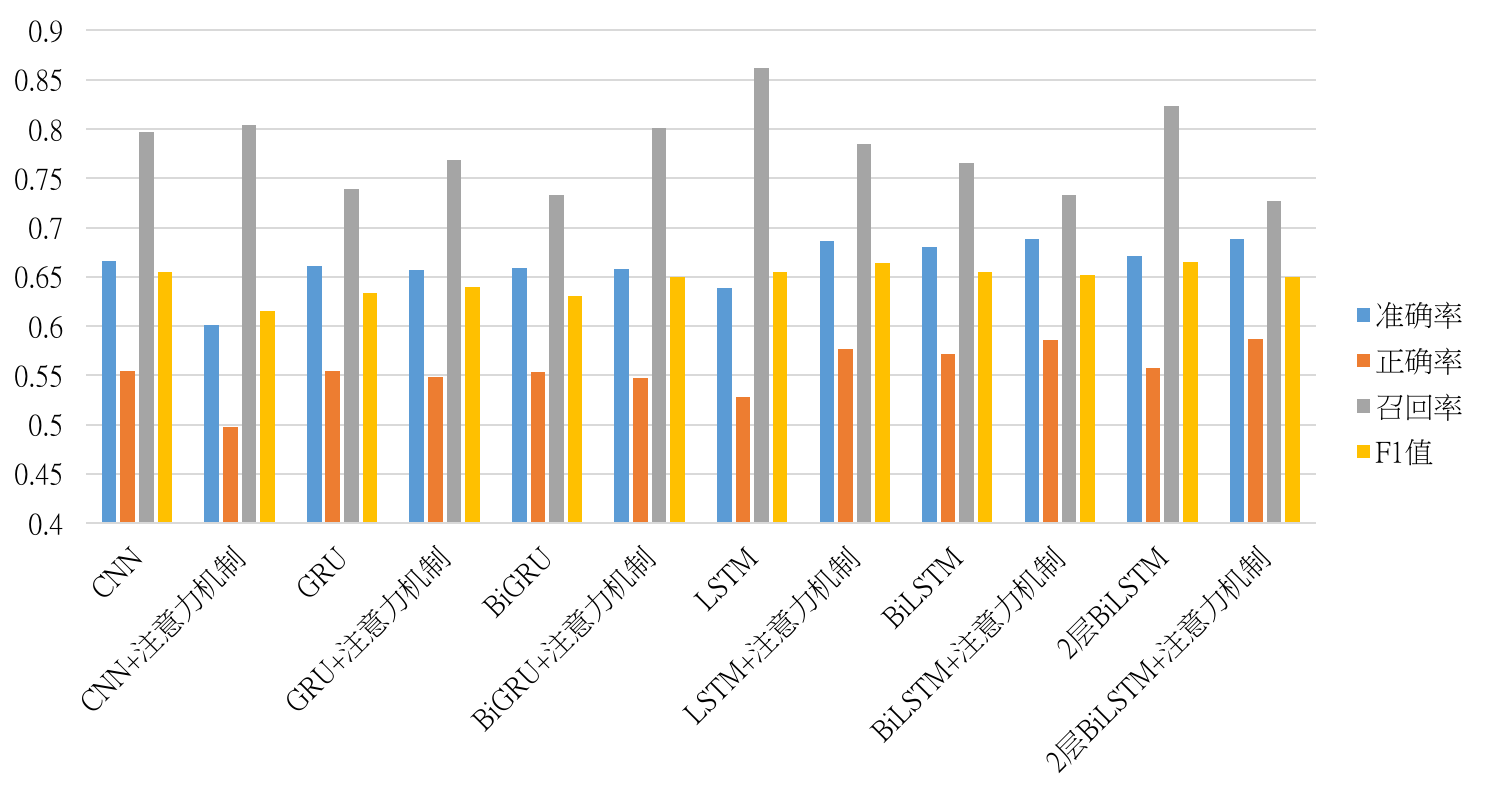
\includegraphics[width=\textwidth]{img/exp_irony_det_A_single_result_bar.png}
  \caption{面向“没有反讽”和“带有反讽”的二分类模型性能}
  \label{fig:exp_irony_det_A_single_result_bar}
\end{figure}

\subsubsection{面向反讽四分类的模型性能分析}
\label{sssec:exp_irony_det_B_base}

对于面向反讽四分类问题,表~\ref{tab:exp_irony_det_B_result}和图~\ref{fig:exp_irony_det_B_single_result_bar}显示不同卷积神经网络和迭归神经网络在测试集上能达到的性能。注意表中的正确率、召回率、F1值均是
各类别对应指标数据的宏平均,对应比赛SemEval2018任务三子任务二关注的主要指标。

对于F1值,BiGRU达到最好的数值(0.4768),其次是2层BiLSTM以及配合注意力机制的2层BiLSTM,与前者的数值差距明显(0.0111)。对于准确率,同样由BiGRU达到最好的数值(0.6722),其次是BiLSTM和2层BiLSTM,和前者的数值差距明显(0.014)。对于正确率,CNN和2层BiLSTM的性能较好(在0.5以上),第三的BiLSTM则在0.49以下。对于召回率,2层BiLSTM配合注意力机制达到最好的0.4864 ,其次的BiGRU和BiLSTM则和前者差距明显(0.0085)。

另外,六组模型在添加注意力机制后正确率、召回率和F1值都有所下降(仅2层BiLSTM的召回率例外),而对于准确率较高的BiGRU、BiLSTM和CNN在添加注意力机制后准确率同样有所下降,可以认为添加注意力机制在此子分类问题中并不没有带来性能提升。

\begin{table}[htb]
  \centering
  \begin{minipage}[t]{\linewidth}
  \caption{面向反讽四分类的模型性能}
  \label{tab:exp_irony_det_B_result}
    \begin{tabularx}{\linewidth}{X|llll}
    \toprule[1.5pt]
    & 准确率 & 正确率 & 召回率 & F1值 \\
    \hline
    CNN & 0.6531 (4) & \bf 0.5090 (1) & 0.4667 (5) & 0.4432 (7) \\ % B_cnn_ek_1554446864
    CNN+注意力机制 & 0.6186 (10) & 0.4467 (7) & 0.4214 (12) & 0.4030 (12) \\ % B_cnn_ek_1554446879
    \hline
    GRU & 0.6148 (12) & 0.4437 (8) & 0.4693 (4) & 0.4476 (5) \\ % B_gru_ek_1554447274
    GRU+注意力机制 & 0.6531 (4) & 0.4253 (10) & 0.4605 (7) & 0.4370 (8) \\ % B_gru_ek_1554447525
    \hline
    BiGRU & \bf 0.6722 (1) & 0.4868 (4) & 0.4779 (2) & \bf 0.4768 (1) \\ % B_bgru_ek_1554447516
    BiGRU+注意力机制 & 0.6301 (9) & 0.4543 (6) & 0.4638 (6) & 0.4497 (4) \\ % B_bgru_ek_1554447697
    \hline
    LSTM & 0.6186 (10) & 0.4313 (9) & 0.4490 (9) & 0.4307 (9) \\ % B_lstm_ek_1554447721
    LSTM+注意力机制 & 0.6416 (6) & 0.4046 (12) & 0.4394 (10) & 0.4148 (11) \\ % B_lstm_ek_1554447878
    \hline
    BiLSTM & 0.6582 (2) & 0.4875 (3) & 0.4537 (8) & 0.4447 (6) \\ % B_blstm_ek_1554447955
    BiLSTM+注意力机制 & 0.6352 (7) & 0.4168 (11) & 0.4386 (11) & 0.4160 (10) \\ % B_blstm_ek_1554448216
    \hline
    2层BiLSTM & 0.6582 (2) & 0.5068 (2) & 0.4762 (3) & 0.4644 (3) \\ % B_nblstm_ek_1554448237
    2层BiLSTM+注意力机制 & 0.6314 (8) & 0.4824 (5) & \bf 0.4864 (1) & 0.4657 (2) \\ % B_nblstm_ek_1554448594
    \bottomrule[1.5pt]
    \end{tabularx}
  \end{minipage}
\end{table}

\begin{figure}[H]
  \centering
  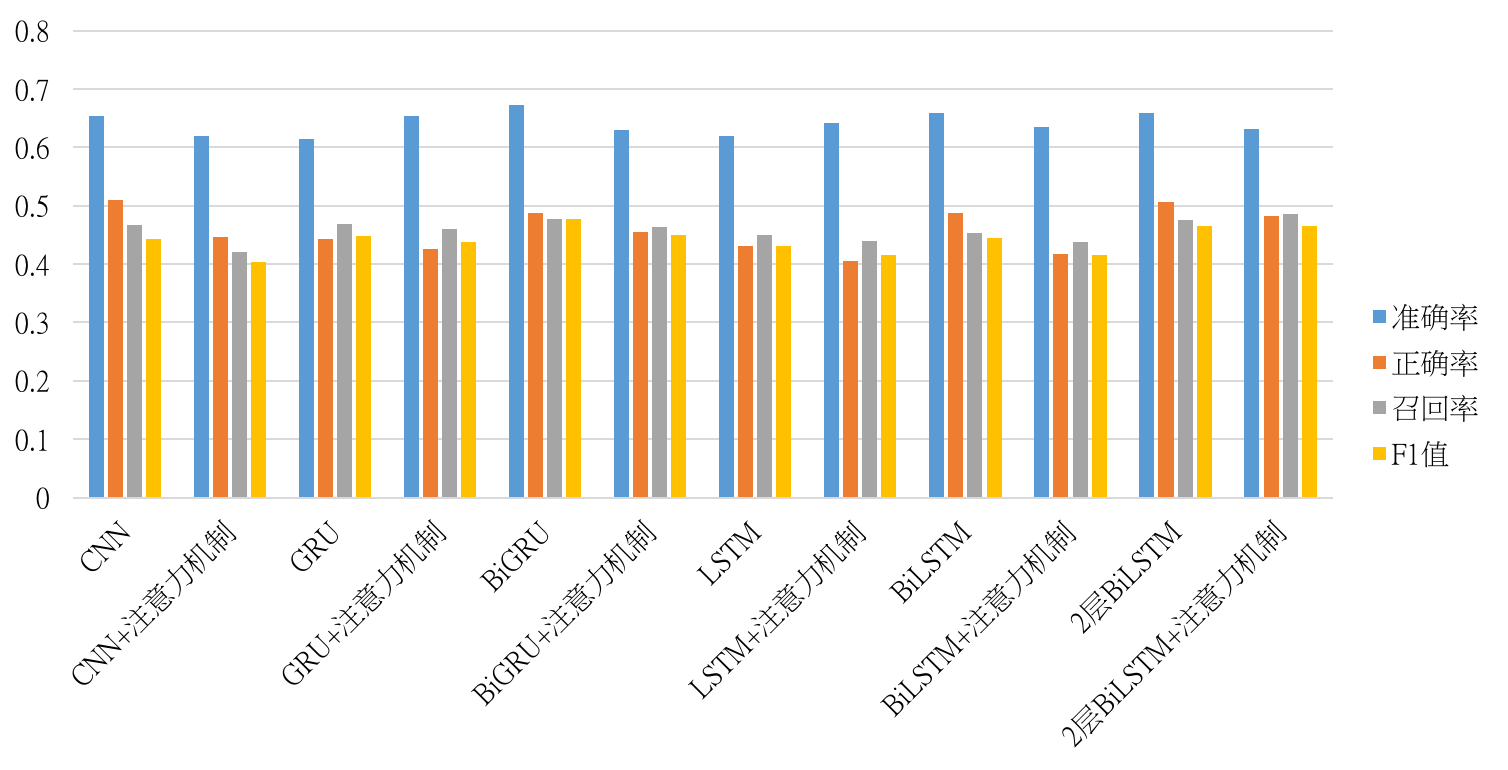
\includegraphics[width=\textwidth]{img/exp_irony_det_B_single_result_bar.png}
  \caption{面向反讽四分类的模型性能}
  \label{fig:exp_irony_det_B_single_result_bar}
\end{figure}

\subsubsection{面向“没有反讽”和“基于相反语义的反讽”二分类的实验结果分析}
\label{sssec:exp_irony_det_Bb01_base}

对于面向“没有反讽”和“基于相反语义的反讽”的二分类问题,表~\ref{tab:exp_irony_det_Bb01_result}和图~\ref{fig:exp_irony_det_Bb01_single_result_bar}显示不同卷积神经网络和迭归神经网络在测试集上能达到的性能。注意表中的正确率、召回率、F1值指两个类别对应指标数据的宏平均。

对于F1值,LSTM配合注意力机制达到最大数值的0.7752 ,其后依次为BiGRU和GRU,和前者差距约较小(0.0047)。对于准确率,同样是LSTM配合注意力机制达到最好的效果(0.8275),其后依次为GRU和BiGRU,和前者差距大(0.0157)。对于正确率,还是 LSTM配合注意力机制的数值最高(0.7717),其后依次为GRU和BiGRU,和前者差距大(0.0151)。对于召回率,数值最高的是BiGRU(0.7993),其次是GRU和LSTM,和前者差距均较小(0.0049)。

总的来说,LSTM配合注意力机制在四项指标中的三项都达到了最好的性能,而各项指标的第二和第三基本上由GRU和BiGRU达到。由配合注意力机制的模型达到最好的性能,这一点和前面各个子分类问题的实验结果都不同,显示注意力机制可能对“基于相反语义的反讽”有相应的建模能力。另外GRU和BiGRU的性能非接近,从数学模型上看,BiGRU比单层GRU多一个把文本反向输入的GRU通道,提高了召回率的同时稍微降低了准确率和正确率,显示反向输入的GRU通道能额外捕足到“基于相反语义的反讽”相关的特征。但相对地BiLSTM在四项指标上都明显低于LSTM,我们认为其中的原因可能有两点,一是LSTM从数学模型上对“基于相反语义的反讽”的特征建模能力较差,二是BiLSTM的模型参数过多而导致对训练集的过拟合。

\begin{table}[htb]
  \centering
  \begin{minipage}[t]{\linewidth}
  \caption{面向“没有反讽”和“基于相反语义的反讽”的二分类各模型性能}
  \label{tab:exp_irony_det_Bb01_result}
    \begin{tabularx}{\linewidth}{X|llll}
    \toprule[1.5pt]
    & 准确率 & 正确率 & 召回率 & F1值 \\
    \hline
    CNN & 0.7991 (5) & 0.7438 (5) & 0.7791 (7) & 0.7562 (5) \\ % Bb01_cnn_ek_1554448736
    CNN+注意力机制 & 0.6829 (12) & 0.6494 (12) & 0.6909 (12) & 0.6470 (12) \\ % Bb01_cnn_ek_1554448788
    \hline
    GRU & 0.8100 (2) & 0.7566 (2) & 0.7944 (2) & 0.7699 (3) \\ % Bb01_gru_ek_1554448924
    GRU+注意力机制 & 0.7677 (9) & 0.7196 (9) & 0.7679 (10) & 0.7303 (9) \\ % Bb01_gru_ek_1554449053
    \hline
    BiGRU & 0.8085 (3) & 0.7565 (3) & \bf 0.7993 (1) & 0.7705 (2) \\ % Bb01_bgru_ek_1554449115
    BiGRU+注意力机制 & 0.7755 (8) & 0.7301 (8) & 0.7831 (5) & 0.7412 (8) \\ % Bb01_bgru_ek_1555407125
    \hline
    LSTM & 0.8053 (4) & 0.7525 (4) & 0.7932 (3) & 0.7661 (4) \\ % Bb01_lstm_ek_1554449707
    LSTM+注意力机制 & \bf 0.8257 (1) & \bf 0.7717 (1) & 0.7791 (7) & \bf 0.7752 (1) \\ % Bb01_lstm_ek_1554449864
    \hline
    BiLSTM & 0.7551 (10) & 0.7169 (10) & 0.7734 (9) & 0.7236 (10) \\ % Bb01_blstm_ek_1554449881
    BiLSTM+注意力机制 & 0.7174 (11) & 0.6909 (11) & 0.7460 (11) & 0.6889 (11) \\ % Bb01_blstm_ek_1554450198
    \hline
    2层BiLSTM & 0.7849 (7) & 0.7339 (7) & 0.7795 (6) & 0.7465 (7) \\ % Bb01_nblstm_ek_1554450231
    2层BiLSTM+注意力机制 & 0.7928 (6) & 0.7421 (6) & 0.7888 (4) & 0.7554 (6) \\ % Bb01_nblstm_ek_1554450448
    \bottomrule[1.5pt]
    \end{tabularx}
  \end{minipage}
\end{table}

\begin{figure}[H]
  \centering
  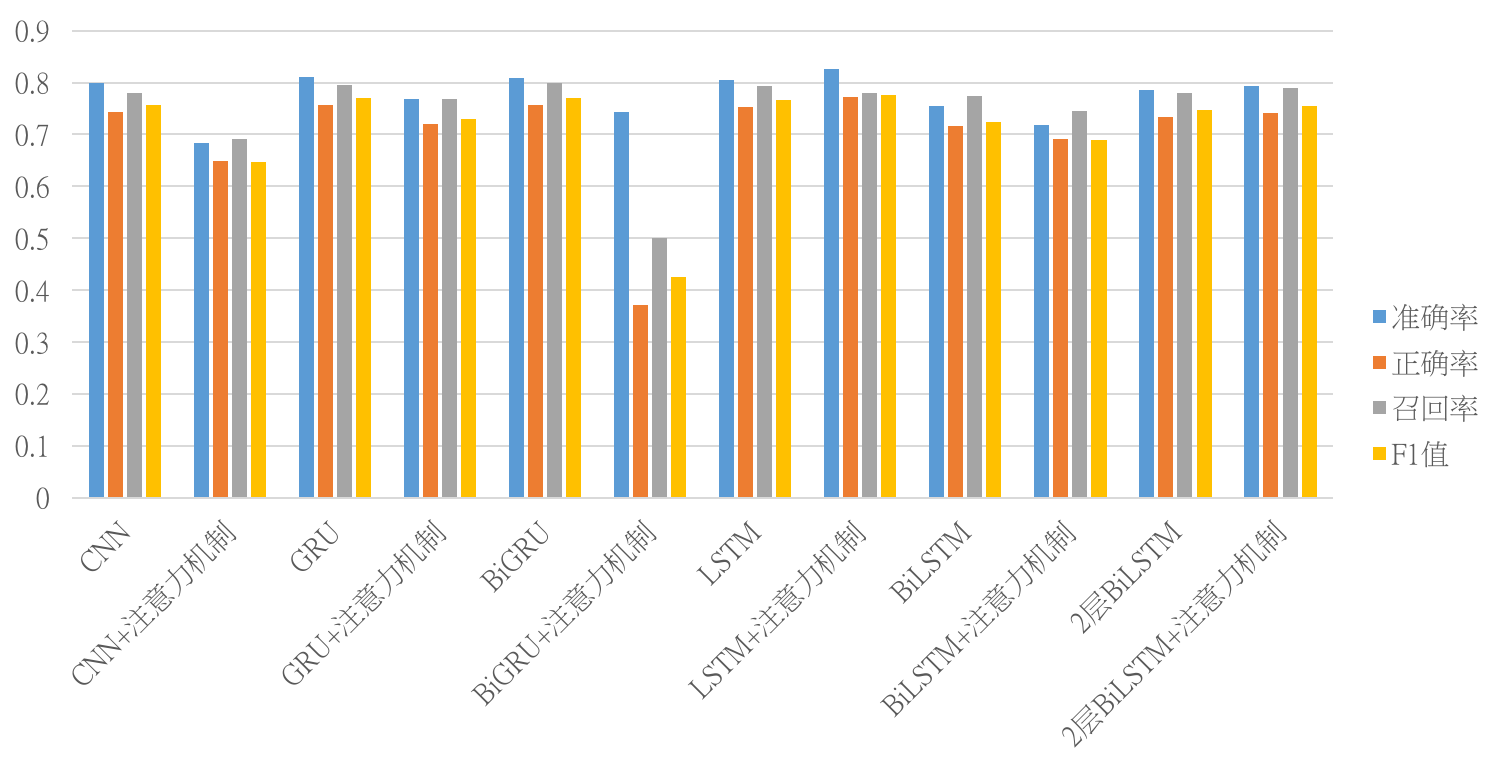
\includegraphics[width=\textwidth]{img/exp_irony_det_Bb01_single_result_bar.png}
  \caption{面向“没有反讽”和“基于相反语义的反讽”的二分类各模型性能}
  \label{fig:exp_irony_det_Bb01_single_result_bar}
\end{figure}

\subsubsection{面向“没有反讽”和“情景反讽”二分类的模型性能分析}
\label{sssec:exp_irony_det_Bb02_base}

对于面向“没有反讽”和“情景反讽”的二分类问题,表~\ref{tab:exp_irony_det_Bb02_result}和图~\ref{fig:exp_irony_det_Bb02_single_result_bar}显示不同卷积神经网络和迭归神经网络在测试集上能达到的性能。注意表中的正确率、召回率、F1值指两个类别对应指标数据的宏平均。

对于F1值和召回率,2层BiLSTM配合注意力机制在这两个指标上都达到了最好的效果(数值分别为0.6924 和 0.6806),其次是2层BiLSTM,第三是单层的BiLSTM配合注意力机制,但后两者在准确率和正确率这两项指标上都排在靠后的位置。而对于准确率和正确率,均由CNN达到最好的效果(数值分别为0.8656和 0.7634),其次是2层BiLSTM配合注意力机制,第三是单层的LSTM。

整体上,2层BiLSTM配合注意力机制在四项指标上的都达到了靠前的效果,显示2层BiLSTM配合注意力机制对“情景反讽”有明显较好的建模能力。另外CNN虽然在准确率和正确率上都达到最好的性能,但由于召回率数值太低导致了F1值明显低于第一的F1值(差距约0.045),显示CNN只对部分“情景反讽”的样本有较好的识别能力,导致了召回率偏低。

\begin{table}[htb]
  \centering
  \begin{minipage}[t]{\linewidth}
  \caption{面向“没有反讽”和“情景反讽”的二分类模型性能}
  \label{tab:exp_irony_det_Bb02_result}
    \begin{tabularx}{\linewidth}{X|llll}
    \toprule[1.5pt]
    & 准确率 & 正确率 & 召回率 & F1值 \\
    \hline
    CNN & \bf 0.8656 (1) & \bf 0.7634 (1) & 0.6167 (7) & 0.6473 (7) \\ % Bb02_cnn_ek_1554450719
    CNN+注意力机制 & 0.8477 (5) & 0.6865 (5) & 0.5917 (11) & 0.6117 (11) \\ % Bb02_cnn_ek_1554450772
    \hline
    GRU & 0.8495 (4) & 0.6942 (4) & 0.6024 (10) & 0.6242 (10) \\ % Bb02_gru_ek_1554450862
    GRU+注意力机制 & 0.8333 (11) & 0.6708 (8) & 0.6556 (4) & 0.6625 (4) \\ % Bb02_gru_ek_1554451013
    \hline
    BiGRU & 0.8423 (6) & 0.6645 (11) & 0.5789 (12) & 0.5951 (12) \\ % Bb02_bgru_ek_1554451047
    BiGRU+注意力机制 & 0.8423 (6) & 0.6825 (6) & 0.6416 (5) & 0.6572 (6) \\ % Bb02_bgru_ek_1554451155
    \hline
    LSTM & 0.8513 (2) & 0.7027 (3) & 0.6372 (6) & 0.6590 (5) \\ % Bb02_lstm_ek_1554451286
    LSTM+注意力机制 & 0.8387 (8) & 0.6676 (10) & 0.6153 (8) & 0.6325 (8) \\ % Bb02_lstm_ek_1554451194
    \hline
    BiLSTM & 0.8351 (10) & 0.6575 (12) & 0.6084 (9) & 0.6243 (9) \\ % Bb02_blstm_ek_1554451336
    BiLSTM+注意力机制 & 0.8369 (9) & 0.6797 (7) & 0.6674 (3) & 0.6731 (3) \\ % Bb02_blstm_ek_1554451401
    \hline
    2层BiLSTM & 0.8262 (12) & 0.6691 (9) & 0.6803 (2) & 0.6743 (2) \\ % Bb02_nblstm_ek_1554451496
    2层BiLSTM+注意力机制 & 0.8513 (2) & 0.7076 (2) & \bf 0.6806 (1) & \bf 0.6924 (1) \\ % Bb02_nblstm_ek_1554451575
    \bottomrule[1.5pt]
    \end{tabularx}
  \end{minipage}
\end{table}

\begin{figure}[H]
  \centering
  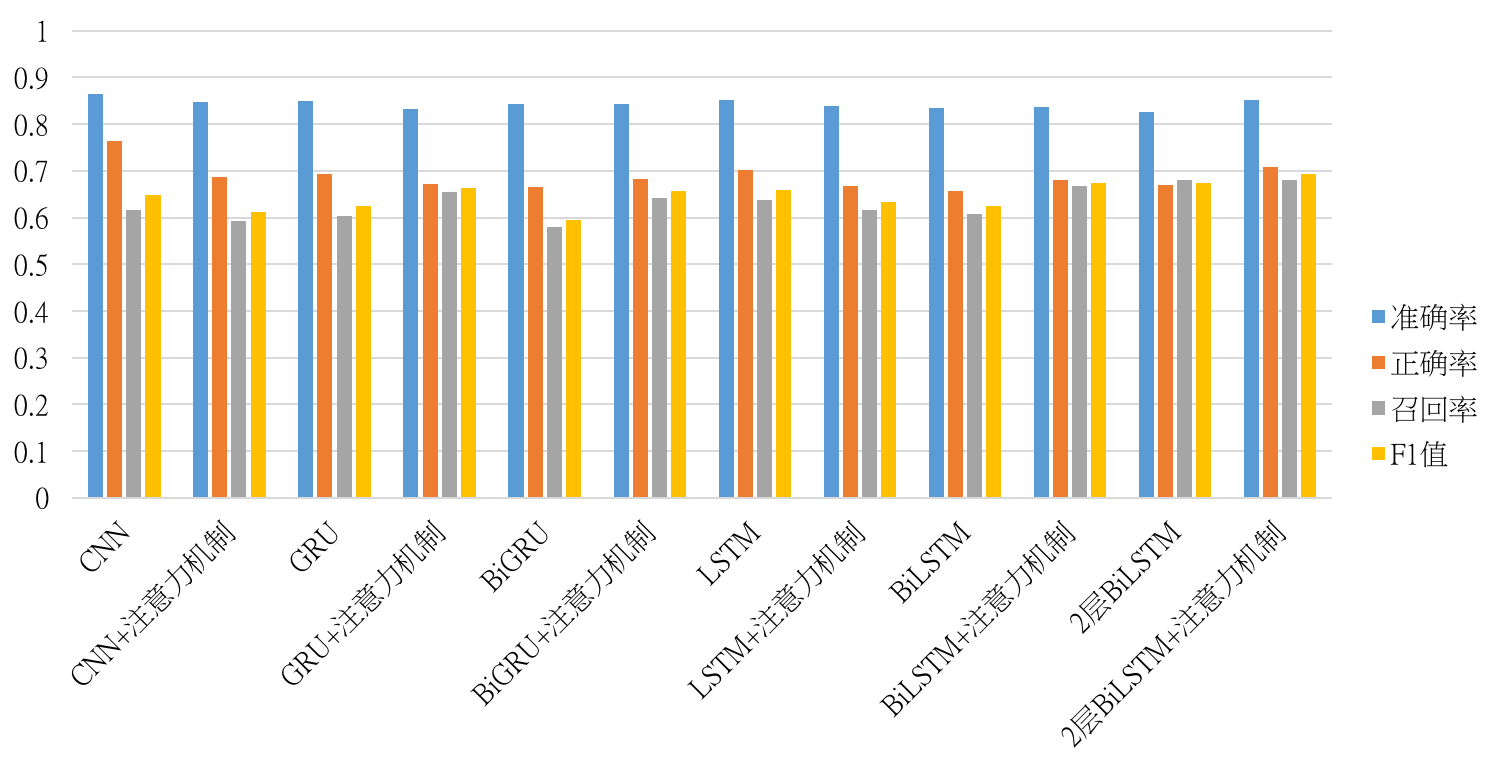
\includegraphics[width=\textwidth]{img/exp_irony_det_Bb02_single_result_bar.png}
  \caption{面向“没有反讽”和“情景反讽”的二分类模型性能}
  \label{fig:exp_irony_det_Bb02_single_result_bar}
\end{figure}

\subsubsection{面向“没有反讽”和“其他反讽”二分类的模型性能分析}
\label{sssec:exp_irony_det_Bb03_base}

对于面向“没有反讽”和“其他反讽”的二分类问题,表~\ref{tab:exp_irony_det_Bb03_result}和图~\ref{fig:exp_irony_det_Bb03_single_result_bar}显示不同卷积神经网络和迭归神经网络在测试集上能达到的性能。注意表中的正确率、召回率、F1值指两个类别对应指标数据的宏平均。

对于F1值,性能最好的是CNN(0.6016),其次是GRU,与前者差距明显(约0.0163),第三为BiLSTM,明显低于CNN的数值(差距约为0.0489)。对于准确率,同样是CNN达到最高的数值(0.8860),其次是GRU配合注意力机制以及LSTM配合注意力机制,在数值上比较接近(差距仅0.0019)。对于正确率,依然是CNN的性能最优(0.7123),第二是GRU配合注意力机制,但和前者差距较明显(约0.0195),第三的GRU则远差于前两者(差距达0.1以上)。 对于召回率,则是GRU的效果最好(0.5836),其次是CNN,与前者差距较小(约0.0055),第三的BiLSTM则和前两者差距较大(达0.0313)。

整体上,CNN在三项指标上的都达到了最好的效果,而在召回率也逼近最好的GRU,显示CNN对“其他反讽”有明显较好的建模能力。对于CNN在准确率和正确率上最佳,这和面向“没有反讽”和“情景反讽”的二分类实验结果相同,这可能有样本量分布有关,“情景反讽”和“其他反讽”的训练样本量(分别为316和205)都远少于“没有反讽”(1923),但CNN对“其他反讽”有较好的建模能力,因此在达到较好召回率的同时达到了最佳的F1值。

\begin{table}[htb]
  \centering
  \begin{minipage}[t]{\linewidth}
  \caption{面向“没有反讽”和“其他反讽”的二分类模型性能}
  \label{tab:exp_irony_det_Bb03_result}
    \begin{tabularx}{\linewidth}{X|llll}
    \toprule[1.5pt]
    & 准确率 & 正确率 & 召回率 & F1值 \\
    \hline
    CNN & \bf 0.8860 (1) & \bf 0.7123 (1) & 0.5781 (2) & \bf 0.6016 (1) \\ % Bb03_cnn_ek_1553500286
    CNN+注意力机制 & 0.7981 (11) & 0.4930 (8) & 0.4934 (11) & 0.4932 (7) \\ % Bb03_cnn_ek_1554453416
    \hline
    GRU & 0.8336 (10) & 0.5873 (3) & \bf 0.5836 (1) & 0.5853 (2) \\ % Bb03_gru_ek_1554452318
    GRU+注意力机制 & 0.8841 (2) & 0.6928 (2) & 0.5070 (7) & 0.4848 (8) \\ % Bb03_gru_ek_1554452300
    \hline
    BiGRU & 0.8411 (8) & 0.5481 (7) & 0.5317 (6) & 0.5353 (6) \\ % Bb03_bgru_ek_1554452373
    BiGRU+注意力机制 & 0.8822 (4) & 0.4419 (11) & 0.4989 (9) & 0.4687 (10) \\ % Bb03_bgru_ek_1554452659
    \hline
    LSTM & 0.8486 (6) & 0.5603 (5) & 0.5360 (4) & 0.5409 (4) \\ % Bb03_lstm_ek_1554452412
    LSTM+注意力机制 & 0.8841 (2) & 0.4421 (10) & 0.5000 (8) & 0.4692 (9) \\ % Bb03_lstm_ek_1554452800
    \hline
    BiLSTM & 0.8430 (7) & 0.5663 (4) & 0.5468 (3) & 0.5527 (3) \\ % Bb03_blstm_ek_1554452497
    BiLSTM+注意力机制 & 0.8822 (4) & 0.4419 (11) & 0.4989 (9) & 0.4687 (10) \\ % Bb03_blstm_ek_1554452804
    \hline
    2层BiLSTM & 0.8355 (9) & 0.5483 (6) & 0.5356 (5) & 0.5393 (5) \\ % Bb03_nblstm_ek_1554452506
    2层BiLSTM+注意力机制 & 0.7944 (12) & 0.4571 (9) & 0.4633 (12) & 0.4600 (12) \\ % Bb03_nblstm_ek_1554452977
    \bottomrule[1.5pt]
    \end{tabularx}
  \end{minipage}
\end{table}

\begin{figure}[H]
  \centering
  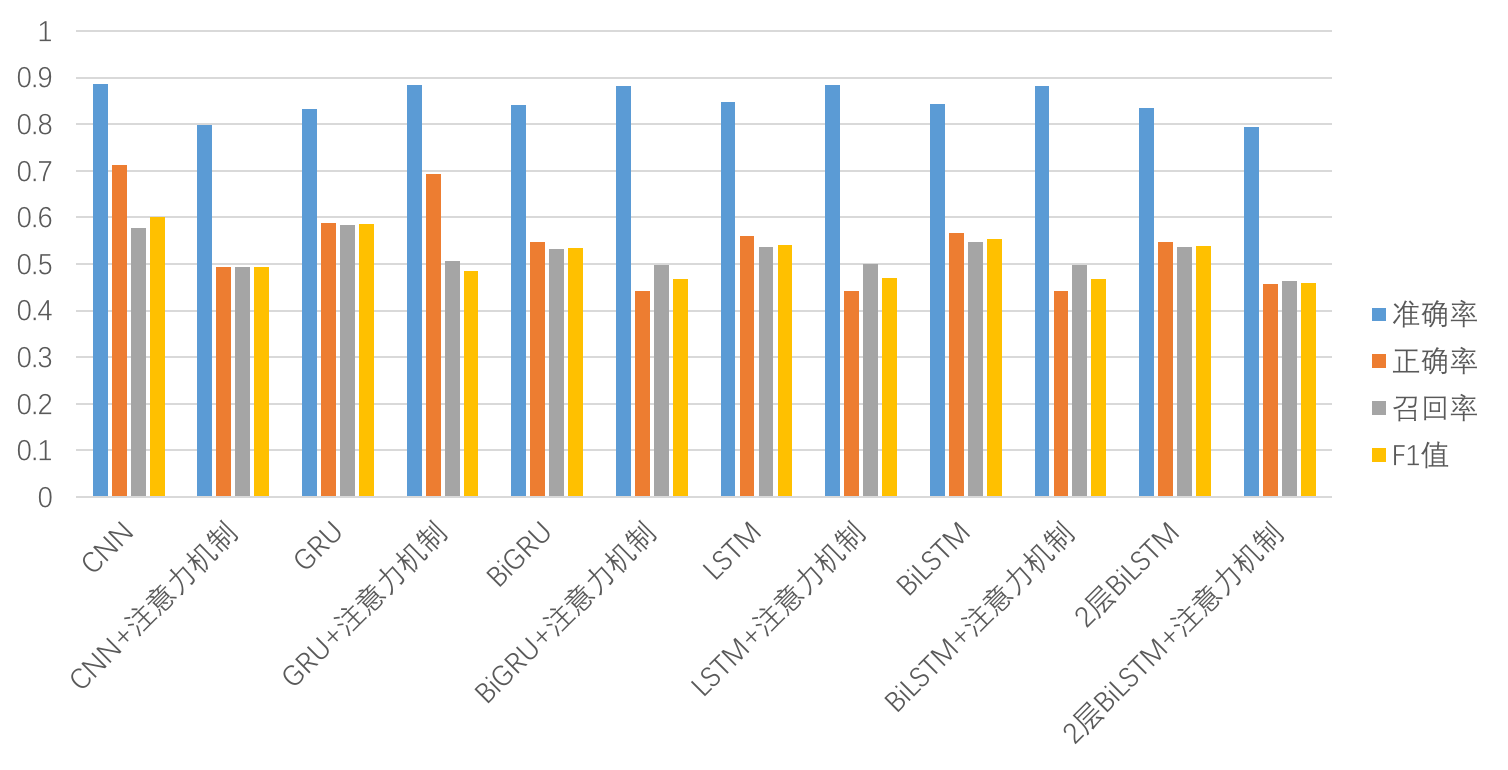
\includegraphics[width=\textwidth]{img/exp_irony_det_Bb03_single_result_bar.png}
  \caption{面向“没有反讽”和“其他反讽”的二分类模型性能}
  \label{fig:exp_irony_det_Bb03_single_result_bar}
\end{figure}

\subsubsection{面向“没有反讽”和“带有反讽”二分类的系统性能分析}

经过前面各章节的分析,我们已经对各个子分类问题中不同模型的性能有大致了解,接下来我们将基于子分类器实现反讽识别系统,并和比赛SemEval-2018任务三的参赛系统比较来评估我们系统的性能水平。

首先对于SemEval-2018任务三的子任务一,即面向“没有反讽”和“带有反讽”的二分类问题,基于章节~\ref{sssec:exp_irony_det_A_base}的实验结果,我们最终选择以F1值最高的2层BiLSTM作为子分类器的模型,按照章节~\ref{ssec:exp_irony_det_model_training}训练出由9个分类器组成的分类器组,按照章节~\ref{sec:exp_irony_det_framework},我由该分类器组的子分类器进行投票来得出一条微博的反讽类别。

表~\ref{tab:exp_irony_det_A_other_comp}显示我们的系统和SemEval-2018任务三子任务一其他参赛系统在测试集上的性能。注意表中的正确率、召回率、F1值均是针对类别“带有反讽”的指标。在SemEval-2018任务三子任务一的最终测试阶段,参赛系统共43个,表中仅显示排名前10(按照F1值排名)或在某项指标排名靠前的参赛系统,其中队伍名称为THU\_HCSI对应我们当时提交的系统,排名第8。

首先观察各项指标上我们系统的性能水平。对于F1值,我们系统的数值为0.7010,对应当时排名第二,略低于第一名的0.7050,显着高于当时第二名的0.6719(差距约0.03)。对于准确率,我们系统的数值为0.7256,对应当时排名第三,和第一名的差距约为0.009。对于正确率,我们系统的数值为0.6176,对应当时排名第五。对于召回率,我们系统的数值为0.8103,对应当时排名第四。总的来说我们的系统在上述四项指标上都达到了靠前的性能,对比我们提交的系统有了明显的提升。

另外对比单个子分类器(即单个2层BiLSTM模型对应的分类器)和整个系统的识别性能,系统在准确率、正确率和F1值都有明显的提升,只有召回率有轻微的下降,显示采用多数投票方法有效基于多个子分类器达到更好的识别性能。

\begin{table}[htb]
  \centering
  \begin{minipage}[t]{\linewidth}
  \caption{SemEval-2018任务三子任务一参赛系统性能} % 共43个参赛系统
  \label{tab:exp_irony_det_A_other_comp}
    \begin{tabularx}{\linewidth}{c|X|llll}
    \toprule[1.5pt]
    排名 & 队伍名称 & 准确率 & 正确率 & 召回率 & F1值 \\
    \hline 
    1 & THU\_NGN & \bf 0.7347 (1) & 0.6304 (4) & 0.8006 (4) & \bf 0.7054 \\
    2 & NTUA-SLP & 0.7321 (2) & 0.6535 (2) & 0.6913 (13) & 0.6719 \\
    3 & WLV & 0.6429 (15) & 0.5317 (20) & 0.8360 (2) & 0.6500 \\
    4 & (无) & 0.6607 (10) & 0.5506 (13) & 0.7878 (7) & 0.6481 \\
    5 & NIHRIO, NCL & 0.7015 (3) & 0.6091 (5) & 0.6913 (13) & 0.6476 \\
    6 & DLUTNLP-1 & 0.6276 (19) & 0.5199 (23) & 0.7974 (5) & 0.6294 \\
    7 & ELiRF-UPV & 0.6110 (23) & 0.5059 (27) & 0.8328 (3) & 0.6294 \\
    8 & \bf THU\_HCSI & 0.6594 (11) & 0.5550 (11) & 0.7138 (10) & 0.6245 \\
    9 & CJ & 0.6671 (8) & 0.5654 (9) & 0.6945 (12) & 0.6234 \\ 
    10 & \#NonDicevoSulSerio & 0.6786 (7) & 0.5831 (8) & 0.6656 (15) & 0.6216 \\
    \hline
    15 & (无) & 0.5651 (31) & 0.4731 (33) & \bf 0.8489 (1) & 0.6076 \\
    \hline
    43 & INGEOTEC-IIMAS & 0.6276 (19) & \bf 0.8800 (1) & 0.0707 (37) & 0.1310 \\
    \hline 
    & 单个分类器 & 0.6709 (8) & 0.5577 (10) & 0.8232 (4) & 0.6649 (3) \\ % A_nblstm_ek_1554346535
    & 我们的系统 & 0.7258 (3) & 0.6176 (5) & 0.8103 (4) & 0.7010 (2) \\
    \bottomrule[1.5pt]
    \end{tabularx}
  \end{minipage}
\end{table}

\subsubsection{面向反讽四分类的系统性能分析}

接下来我们分析面向反讽四分类的系统性能,对应SemEval-2018任务三的子任务二。按照章节~\ref{sec:exp_irony_det_framework},我们的反讽四分类系统涉及四个子分类问题。

对于和原问题相同的反讽四分类,根据章节~\ref{sssec:exp_irony_det_B_base}的实验结果,我们采用BiGRU的模型作为第一组分类器。对于面向“没有反讽”和“基于相反语义的反讽”的二分类问题,按照章节~\ref{sssec:exp_irony_det_Bb01_base}的实验结果,我们采用LSTM配合注意力机制作为第二组分类器的模型。对于“没有反讽”和“情景反讽”的二分类问题,按照章节~\ref{sssec:exp_irony_det_Bb02_base}的实验结果,我们采用2层BiLSTM+注意力机制作为第三组分类器的模型。对于“没有反讽”和“其他反讽”的二分类问题,按照章节~\ref{sssec:exp_irony_det_Bb03_base}的实验结果,我们采用CNN作为第四组分类器的模型。按照章节~\ref{ssec:exp_irony_det_model_training},我们基于选定的模型分别为每个分类器组训练5个分类器。

最后按照章节~\ref{sec:exp_irony_det_framework}中的设计的流程,经过各个组的投票结果逐步调整预测结果,最终得出一条微博的细分反讽类别。对于系统中对第二、三、四个分类器组需要配置的与置信度相关的参数$thr_2$、$thr_3$和$thr_4$ ,我们均设置为3,即完全相信第二、三、四个分类器组中过半数的投票结果。

表~\ref{tab:exp_irony_det_B_other_comp}显示我们的系统和SemEval-2018任务三子任务二其他参赛系统在测试集上的性能。注意表中的正确率、召回率、F1值均是针对各类别对应指标数据的宏平均。在SemEval-2018任务三子任务二的最终测试阶段,参赛系统共31个,表中仅显示排名前10(按照F1值排名)的参赛系统,而我们当时并未参与子任务二。
 
首先观察各项指标上我们系统的性能水平。对于F1值,我们系统的数值为0.5205,对应当时排名第一,显着高于当时的第一名的0.5074。对于准确率,我们系统的数值为0.6939,对应当时准确率排名第二,和最高数值的0.7321差距较大。对于正确率,我们系统的数值为0.6003,对应当时正确率排名第一,显着高于当时最高0.5768的正确率。
对于召回率,我们系统的数值为0.5241,对应当时召回率排名第二,和最高数值的0.5414差距较大。

总的来说我们的系统在上述四项指标上都达到了前二的性能,并在主要评价指标F1值和正确率上显着超过了当时的第一名。对比第一名的系统,我们系统的准确率要低于前者,而正确率和召回率都比它高,可以推断我们的系统成功召回了较多“带有反讽”的细分类别的样本,但同时把靠多真实标签为“没有反讽”的样本误判为“带有反讽”的细分类别。对于以较低的准确率换来较高的F1值,这与各类别的样本数量分布有关,由于“情景反讽”和“其他反讽”的样本量在测试集中占比较小而“没有反讽”的占比较大,以误判较多“没有反讽”的样本为代价召回更多“情景反讽”和“其他反讽”的样本能够明显提高最终的F1值。

\begin{table}[htb]
  \centering
  \begin{minipage}[t]{\linewidth}
  \caption{SemEval-2018任务三子任务二参赛系统性能} % 共31个参赛系统
  \label{tab:exp_irony_det_B_other_comp}
    \begin{tabularx}{\linewidth}{c|X|llll}
    \toprule[1.5pt]
    排名 & 队伍名称 & 准确率 & 正确率 & 召回率 & F1值 \\
    \hline 
    1 & (无) & \bf 0.7321 (1) & \bf 0.5768 (1) & 0.5044 (4) & 0.5074 \\
    2 & NTUA-SLP & 0.6518 (4) & 0.4959 (4) & 0.5124 (2) & 0.4959 \\
    3 & \bf THU\_NGN & 0.6046 (9) & 0.4860 (6) & \bf 0.5414 (1) & 0.4947 \\
    4 & (无) & 0.6033 (10) & 0.4660 (7) & 0.5058 (3) & 0.4743 \\
    5 & NIHRIO, NCL & 0.6594 (3) & 0.5446 (2) & 0.4475 (5) & 0.4437 \\
    6 & Random Decision Syntax Trees & 0.6327 (6) & 0.4868 (5) & 0.4388 (8) & 0.4352 \\
    7 & ELiRF-UPV & 0.6327 (6) & 0.4123 (12) & 0.4404 (7) & 0.4211 \\
    8 & WLV & 0.6709 (2) & 0.4311 (10) & 0.4149 (9) & 0.4153 \\
    9 & \#NonDicevoSulSerio & 0.5446 (18) & 0.4087 (15) & 0.4410 (6) & 0.4131 \\
    10 & INGEOTEC-IIMAS & 0.6441 (5) & 0.5017 (3) & 0.3850 (15) & 0.4055 \\
    \hline
    & 我们的系统 & 0.6939 (2) & \bf 0.6003 (1) & 0.5241 (2) & \bf 0.5205 (1) \\
    \bottomrule[1.5pt]
    \end{tabularx}
  \end{minipage}
\end{table}

另外,由于我们的系统在经过每一步决策后的中间结果都可认作为一组预测结果,我们观察了每组中间结果在测试集上的性能。表~\ref{tab:exp_irony_det_B_ensemble_result}显示我们系统的中间结果在测试集上的各项指标,注意表中的正确率、召回率、F1值均是针对各类别对应指标数据的宏平均。

表中的第一行“中间结果I”对应直接由一组四分类器进行多数投票的识别结果,第二行“中间结果II”是基于第二个分类器组的投票对被判定为“没有反讽”和“基于相反语义的反讽”的样本重新进行二分类的识别结果,可见各项指标都有所提升。再对比中间结果I和中间结果II的混淆矩阵(分别对应表~\ref{tab:exp_irony_det_B_conf_mat_1}和表~\ref{tab:exp_irony_det_B_conf_mat_2})可以发现正确召回了9个“没有反讽”的样本,同时误判了3个原本识别正确的“基于相反语义的反讽”的样本,故整体准确率有所上升。

表中的第三行“中间结果III”是基于第三个分类器组的投票对被判定为“没有反讽”和“情景反讽”的样本重新进行二分类的识别结果,可见准确率不变,正确率稍微下降,同时召回率有了明显提高,导致F1值也明显提高。再对比中间结果II和中间结果III的混淆矩阵(分别对应表~\ref{tab:exp_irony_det_B_conf_mat_2}和表~\ref{tab:exp_irony_det_B_conf_mat_3})可以发现误判了14个原本识别正确的“没有反讽”的样本,同时正确召回了14个“情景反讽”的样本,所以准确率不变,但由于“情景反讽”的样本总量较少而“没有反讽”的样本总量较多,“情景反讽”的召回率显着上升而拔高了宏平均的召回率,这也显示了对于宏平均的指标,关注样本量少的类别能在数值上带来明显提升。

表中的最底一行的“最终结果”是基于第四个分类器组的投票对被判定为“没有反讽”和“其他反讽”的样本重新进行二分类的识别结果,可见各项指标都有所提高。再对比中间结果III和最终结果的混淆矩阵(分别对应表~\ref{tab:exp_irony_det_B_conf_mat_3}和表~\ref{tab:exp_irony_det_B_conf_mat_4})可以发现这一步把5个被误判为“其他反讽”的样本都改成了“没有反讽”,虽然其中只有2个样本的真实标签为“没有反讽”,但由于被识别为“其他反讽”的样本少,明显提高了“其他反讽”的正确率。

总结以上分析结合,我们设计的多步决策框架有效运用多个子分类问题对应的分类器组来提高整个系统的识别性能,其中核心原因有以两点:

\begin{itemize}

\item 从原始问题中提取出子分类问题,并只针对这部份数据训练分类器,由于这些分类器只关注一个比原始问题更简单的子问题,所以他们对局部数据的识别效果更好。另外各个子分类器组的模型不同,可以针对不同类别的数据选用最合适的模型,从章节~\ref{sssec:exp_irony_det_Bb01_base}、\ref{sssec:exp_irony_det_Bb02_base}、\ref{sssec:exp_irony_det_Bb03_base}可以看出虽然“基于相反语义的反讽”、“情景反讽”和“其他反讽”都是“带有反讽”的细分类别,但在子分类问题中各个模型的性能不同,显示这些类别背后和反讽相关的语言特征也不同,那么尝试使用单个数学模型同时拟合并区分这些类别的数据就并不合理,而把原始问题拆解成多个子分类问再透过多步决策来调整识别结果就有效融合不同数学模型的建模能力。

\item 针对宏平均指标以及样本量不均匀的情况选择出合适的子分类问题。原本的四分类问题可以被拆解出多种子分类问题,但我们的系统里只考虑了“没有反讽”和各个“带有反讽”子类两两组合的二分类问题,原因在于“没有反讽”一类的样本量显着多于其他类别,从中间结果I对应的混淆矩阵(对应表~\ref{tab:exp_irony_det_B_conf_mat_1})也可以看出这些类别最容易被误判为“没有反讽”,因此针对“没有反讽”和其他类别之间的识别结果进行调整能带来更显着的性能提升。而每一步只考虑两个类别的原因和宏平均指标紧密相关,在样本量不均匀的数据集上,宏平均指标偏低的常见原因是样本量少的类别的指标数值太低,进而拉低了宏平均的数值,因此对“没有反讽”和各个“带有反讽”子类两两进行调整,有较大可能提高后者的指标,从而提高宏平均的数值。

\end{itemize}

\begin{table}[htb]
  \centering
  \begin{minipage}[t]{0.8\linewidth}
  \caption{四分类反讽识别系统最终识别结果和中间结果的性能}
  \label{tab:exp_irony_det_B_ensemble_result}
    \begin{tabularx}{\linewidth}{X|cccc}
    \toprule[1.5pt]
    & 准确率 & 正确率 & 召回率 & F1值 \\
    \hline
    中间结果I & 0.6837 & 0.5606 & 0.4891 & 0.4913 \\
    中间结果II & 0.6913 & 0.5655 & 0.4893 & 0.4949 \\
    中间结果III & 0.6913 & 0.5587 & 0.5231 & 0.5179 \\
    \hline
    最终结果 & \bf 0.6939 & \bf 0.6003 & \bf 0.5241 & \bf 0.5205 \\
    \bottomrule[1.5pt]
    \end{tabularx}
  \end{minipage}
\end{table}

\begin{table}[]
  \centering
  \begin{minipage}[t]{0.8\linewidth}
  \caption{
    \label{tab:exp_irony_det_B_conf_mat_1}
    反讽四分类测试集上中间结果I对应的混淆矩阵
  }
  \begin{tabularx}{\linewidth}{c|c|cccc}
  \toprule[1.5pt]
  \multicolumn{2}{c|}{\multirow{2}{*}} & \multicolumn{4}{c}{预测标签}    \\
  \cline{3-6} 
  \multicolumn{2}{c|}{}
    & 没有反讽 & 反义反讽 & 情景反讽 & 其他反讽  \\
  \hline
  \multirow{4}{*}{真实标签}
    & 没有反讽 & 380 & 73 & 13 & 7 \\
    & 反义反讽 & 36 & 125 & 3 & 0 \\
    & 情景反讽 & 44 & 13 & 25 & 3 \\
    & 其他反讽 & 41 & 10 & 5 & 6 \\
  \bottomrule[1.5pt]
  \end{tabularx}
  \end{minipage}
\end{table}

\begin{table}[]
  \centering
  \begin{minipage}[t]{0.8\linewidth}
  \caption{
    \label{tab:exp_irony_det_B_conf_mat_2}
    反讽四分类测试集上中间结果II对应的混淆矩阵
  }
  \begin{tabularx}{\linewidth}{c|c|cccc}
  \toprule[1.5pt]
  \multicolumn{2}{c|}{\multirow{2}{*}} & \multicolumn{4}{c}{预测标签}    \\
  \cline{3-6} 
  \multicolumn{2}{c|}{}
    & 没有反讽 & 反义反讽 & 情景反讽 & 其他反讽  \\
  \hline
  \multirow{4}{*}{真实标签}
    & 没有反讽 & 389 & 64 & 13 & 7 \\ 
    & 反义反讽 & 39 & 122 & 3 & 0 \\
    & 情景反讽 & 47 & 10 & 25 & 3 \\
    & 其他反讽 & 39 & 12 & 5 & 6 \\
  \bottomrule[1.5pt]
  \end{tabularx}
  \end{minipage}
\end{table}

\begin{table}[]
  \centering
  \begin{minipage}[t]{0.8\linewidth}
  \caption{
    \label{tab:exp_irony_det_B_conf_mat_3}
    反讽四分类测试集上中间结果III对应的混淆矩阵
  }
  \begin{tabularx}{\linewidth}{c|c|cccc}
  \toprule[1.5pt]
  \multicolumn{2}{c|}{\multirow{2}{*}} & \multicolumn{4}{c}{预测标签}    \\
  \cline{3-6} 
  \multicolumn{2}{c|}{}
    & 没有反讽 & 反义反讽 & 情景反讽 & 其他反讽  \\
  \hline
  \multirow{4}{*}{真实标签}
    & 没有反讽 & 375 & 64 & 27 & 7 \\
    & 反义反讽 & 35 & 122 & 7 & 0 \\
    & 情景反讽 & 33 & 10 & 39 & 3 \\
    & 其他反讽 & 38 & 12 & 6 & 6 \\
  \bottomrule[1.5pt]
  \end{tabularx}
  \end{minipage}
\end{table}

\begin{table}[]
  \centering
  \begin{minipage}[t]{0.8\linewidth}
  \caption{
    \label{tab:exp_irony_det_B_conf_mat_4}
    反讽四分类测试集上最终识别结果对应的混淆矩阵
  }
  \begin{tabularx}{\linewidth}{c|c|cccc}
  \toprule[1.5pt]
  \multicolumn{2}{c|}{\multirow{2}{*}} & \multicolumn{4}{c}{预测标签}    \\
  \cline{3-6} 
  \multicolumn{2}{c|}{}
    & 没有反讽 & 反义反讽 & 情景反讽 & 其他反讽  \\
  \hline
  \multirow{4}{*}{真实标签}
    & 没有反讽 & 377 & 64 & 27 & 5 \\
    & 反义反讽 & 35 & 122 & 7 & 0 \\ 
    & 情景反讽 & 36 & 10 & 39 & 0 \\
    & 其他反讽 & 38 & 12 & 6 & 6 \\
  \bottomrule[1.5pt]
  \end{tabularx}
  \end{minipage}
\end{table}

\subsection{错误分析}
\label{ssec:exp_irony_det_error_analysis}

本节中,我们将对系统错误识别的样本进行观察,分析其中的原因,从而对问题有更进入的了解以及下一步的改进方向。以下使用的例子均参照表~\ref{tab:semeval_2018_task3_error}。

\begin{itemize}

\item {\bf 词组语义倾向识别}。参考例子1,其中“blame”表示指责,在字面意思上有明显的负面情感倾向,而“XXX of the Year”意思为年度最佳的某某,整个词组带有正面情感倾向,故和前者对比得出原微博带有“基于相反语义的反讽”。关键在于词组“XXX of the Year”在逐字解读时没有明显的情感倾向,这也是文本意图识别中常见的问题之一。那么要使得基于人工神经网络的系统有能力识别词组的语义倾向,其必要条件之一是在训练集中出现过类似的词组,对此可以透过收集更多训练样本来保证对常用词组的复盖率,但对于不常用或新出现的词组则需要额外引语言知识。

\item {\bf 场景描述识别}。参考例子2,用户表示他在担任校医当天发烧了,其中“担任校医”为场景,“发烧”的发生和对“担任校医”的预期相反,因此属于“情景反讽”,这种预期的相反也表现在“nurse”和“fever”的字面意思,而该样本被我们的系统误判为“基于相反语义的反讽”。同样地对于例子3,用户表示工作怎么能在他没有上班的期间完成,其中“没有上班”为场景,“工作完成”的发生和对“没有上班”的预期相反,因此属于“情景反讽”,同时在字面上“work get done”和“off week”又表现出某种语义的相反,因而被系统为识别为“基于相反语义的反讽”。再观察我们系统在测试集上的混淆矩阵(表~\ref{tab:exp_irony_det_B_conf_mat_4}),可以发现有相当一部分“情景反讽”的样本被误判为“基于相反语义的反讽”,由此我们推断其中的原因之一在于部分“情景反讽”的样本确实存在相反语义的内容,而从包含相反语义的内容中识别出“场景”会是召回这部分样本的关键。

\item {\bf 一词多义}。参考例子4,“\#Starbucks”是一家国际连锁咖啡店的名字,而在咖啡店的场景下,“tall”指咖啡杯一种大小,“blonde”为该店某个咖啡系统列的名称,而在日常生活常情景中,“tall blonde”还有高挑金发女子的意思,即出现一词多义,而后者的意思在咖啡店场景下发生就产生了和预期相反的效果,因此属于“情景反讽”。反之,要识别出例子中的“情景反讽”就要求系统认识到“tall blonde”具有咖啡以外的意思。由于在我们的模型中,每个单词都以一个固定的词向量表示,因此无法表示单词的一词多义,更无法对多种含意的词组进行建模。直观上,在模型中考虑一词多义是解决方法之一。另外,让系统能够将“Starbucks”和咖啡关联起来则要求在训练集上有包含对应信息的样本。

\item {\bf 信息不足}。参考例子5,“clashupdate”并非标准英语单词或网络上的常用单词,后面紧接着一个超链接,仅凭字面意思无法理解用户要表达的意思。而访问该链接对应网页会发现插图为游戏“Clash of Clans”的更新提示,所以文本中的“clashupdate”应对应“clash update”,依然没有表示反讽的意思,但我们发现原微博的完整文本内容为“clashupdate \#not”,其中“\#not”在微博反讽识别的研究中是最常被用于对微博进行自动标注的井号标签之一,被组织者在准备数据集时故意过滤了。在比赛中,尝试找到微博原文有悖于组织者的初衷(不依赖井号标签进行分类),但在具体应用场景中,若要正确判断这些样本就可以考虑分析链接中的评论,这也对应下一章中探讨引入上下文的意图识别。

\end{itemize}

\begin{table}[htb]
  \centering
  \begin{minipage}[t]{\linewidth} % 如果想在表格中使用脚注,minipage是个不错的办法
  \caption{反讽识别子任务二中被系统误判的样本例子}
  \label{tab:semeval_2018_task3_error}
  \begin{tabularx}{\linewidth}{c|l|X}
    \toprule[1.5pt]
    编号 & 反讽类别 & 微博 \\
    \hline
    1 & 反义反讽 & I blame my mom. Mother of the Year \\
    2 & 情景反讽 & So I'm the school nurse today. And I have a fever. \\
    3 & 情景反讽 & Also it is funny how things at work get done when I'm on my off week \\
    4 & 情景反讽 & Just walked in to \#Starbucks and asked for a “tall blonde” Hahahaha \\
    5 & 其他反讽 & clashupdate http://t.co/1bFOsIwnI5 \\
    \bottomrule[1.5pt]
  \end{tabularx}
  \end{minipage}
\end{table}

\section{本章小结}

在本章中我们研究了面向微博的反讽识别,基于国际比赛SemEval-2018任务三的两个子任务进行了多组实验。对于子任务一,即“没有反讽”和“带有反讽”二分类,我们的模型达到了当时靠前的效果,和我们当时提交的系统性能相比有了显着的提升。对于子任务二,即“没有反讽”、“基于相反语义的反讽”、“情景反讽”和“其他反讽”四分类,我们提出了一个多步决策的反讽识别系统,从原始问题中选出四个子分类问题,再分别选择合适的模型训练出对应的子分类器组,最后透过多步决策融合这些模型的识别结果。实验结果显示我们的系统在核心指标的F1值上显着高于当时的第一名,而在其他三个指标上均达到仅次于当时第一的性能,验证了我们多步决策框架的有效性。
